\documentclass[twoside]{book}

% Packages required by doxygen
\usepackage{fixltx2e}
\usepackage{calc}
\usepackage{doxygen}
\usepackage[export]{adjustbox} % also loads graphicx
\usepackage{graphicx}
\usepackage[utf8]{inputenc}
\usepackage{makeidx}
\usepackage{multicol}
\usepackage{multirow}
\PassOptionsToPackage{warn}{textcomp}
\usepackage{textcomp}
\usepackage[nointegrals]{wasysym}
\usepackage[table]{xcolor}

% Font selection
\usepackage[T1]{fontenc}
\usepackage[scaled=.90]{helvet}
\usepackage{courier}
\usepackage{amssymb}
\usepackage{sectsty}
\renewcommand{\familydefault}{\sfdefault}
\allsectionsfont{%
  \fontseries{bc}\selectfont%
  \color{darkgray}%
}
\renewcommand{\DoxyLabelFont}{%
  \fontseries{bc}\selectfont%
  \color{darkgray}%
}
\newcommand{\+}{\discretionary{\mbox{\scriptsize$\hookleftarrow$}}{}{}}

% Page & text layout
\usepackage{geometry}
\geometry{%
  a4paper,%
  top=2.5cm,%
  bottom=2.5cm,%
  left=2.5cm,%
  right=2.5cm%
}
\tolerance=750
\hfuzz=15pt
\hbadness=750
\setlength{\emergencystretch}{15pt}
\setlength{\parindent}{0cm}
\setlength{\parskip}{3ex plus 2ex minus 2ex}
\makeatletter
\renewcommand{\paragraph}{%
  \@startsection{paragraph}{4}{0ex}{-1.0ex}{1.0ex}{%
    \normalfont\normalsize\bfseries\SS@parafont%
  }%
}
\renewcommand{\subparagraph}{%
  \@startsection{subparagraph}{5}{0ex}{-1.0ex}{1.0ex}{%
    \normalfont\normalsize\bfseries\SS@subparafont%
  }%
}
\makeatother

% Headers & footers
\usepackage{fancyhdr}
\pagestyle{fancyplain}
\fancyhead[LE]{\fancyplain{}{\bfseries\thepage}}
\fancyhead[CE]{\fancyplain{}{}}
\fancyhead[RE]{\fancyplain{}{\bfseries\leftmark}}
\fancyhead[LO]{\fancyplain{}{\bfseries\rightmark}}
\fancyhead[CO]{\fancyplain{}{}}
\fancyhead[RO]{\fancyplain{}{\bfseries\thepage}}
\fancyfoot[LE]{\fancyplain{}{}}
\fancyfoot[CE]{\fancyplain{}{}}
\fancyfoot[RE]{\fancyplain{}{\bfseries\scriptsize Generated by Doxygen }}
\fancyfoot[LO]{\fancyplain{}{\bfseries\scriptsize Generated by Doxygen }}
\fancyfoot[CO]{\fancyplain{}{}}
\fancyfoot[RO]{\fancyplain{}{}}
\renewcommand{\footrulewidth}{0.4pt}
\renewcommand{\chaptermark}[1]{%
  \markboth{#1}{}%
}
\renewcommand{\sectionmark}[1]{%
  \markright{\thesection\ #1}%
}

% Indices & bibliography
\usepackage{natbib}
\usepackage[titles]{tocloft}
\setcounter{tocdepth}{3}
\setcounter{secnumdepth}{5}
\makeindex

% Hyperlinks (required, but should be loaded last)
\usepackage{ifpdf}
\ifpdf
  \usepackage[pdftex,pagebackref=true]{hyperref}
\else
  \usepackage[ps2pdf,pagebackref=true]{hyperref}
\fi
\hypersetup{%
  colorlinks=true,%
  linkcolor=blue,%
  citecolor=blue,%
  unicode%
}

% Custom commands
\newcommand{\clearemptydoublepage}{%
  \newpage{\pagestyle{empty}\cleardoublepage}%
}

\usepackage{caption}
\captionsetup{labelsep=space,justification=centering,font={bf},singlelinecheck=off,skip=4pt,position=top}

%===== C O N T E N T S =====

\begin{document}

% Titlepage & ToC
\hypersetup{pageanchor=false,
             bookmarksnumbered=true,
             pdfencoding=unicode
            }
\pagenumbering{roman}
\begin{titlepage}
\vspace*{7cm}
\begin{center}%
{\Large Bulk }\\
\vspace*{1cm}
{\large Generated by Doxygen 1.8.11}\\
\end{center}
\end{titlepage}
\clearemptydoublepage
\tableofcontents
\clearemptydoublepage
\pagenumbering{arabic}
\hypersetup{pageanchor=true}

%--- Begin generated contents ---
\chapter{Namespace Index}
\section{Namespace List}
Here is a list of all namespaces with brief descriptions\+:\begin{DoxyCompactList}
\item\contentsline{section}{\hyperlink{namespace_utils}{Utils} }{\pageref{namespace_utils}}{}
\end{DoxyCompactList}

\chapter{Hierarchical Index}
\section{Class Hierarchy}
This inheritance list is sorted roughly, but not completely, alphabetically\+:\begin{DoxyCompactList}
\item \contentsline{section}{Console\+Logger}{\pageref{struct_console_logger}}{}
\item \contentsline{section}{Event\+Dispatcher}{\pageref{class_event_dispatcher}}{}
\begin{DoxyCompactList}
\item \contentsline{section}{Bulk}{\pageref{class_bulk}}{}
\end{DoxyCompactList}
\item \contentsline{section}{File\+Logger}{\pageref{struct_file_logger}}{}
\item \contentsline{section}{I\+Expression}{\pageref{struct_i_expression}}{}
\begin{DoxyCompactList}
\item \contentsline{section}{Command}{\pageref{struct_command}}{}
\item \contentsline{section}{Group}{\pageref{struct_group}}{}
\end{DoxyCompactList}
\item \contentsline{section}{I\+Interpreter\+State}{\pageref{class_i_interpreter_state}}{}
\begin{DoxyCompactList}
\item \contentsline{section}{Infinit\+Sequence}{\pageref{class_infinit_sequence}}{}
\item \contentsline{section}{Sequence}{\pageref{class_sequence}}{}
\end{DoxyCompactList}
\end{DoxyCompactList}

\chapter{Class Index}
\section{Class List}
Here are the classes, structs, unions and interfaces with brief descriptions\+:\begin{DoxyCompactList}
\item\contentsline{section}{\hyperlink{class_bulk}{Bulk} }{\pageref{class_bulk}}{}
\item\contentsline{section}{\hyperlink{struct_command}{Command} }{\pageref{struct_command}}{}
\item\contentsline{section}{\hyperlink{struct_console_logger}{Console\+Logger} }{\pageref{struct_console_logger}}{}
\item\contentsline{section}{\hyperlink{class_event_dispatcher}{Event\+Dispatcher} }{\pageref{class_event_dispatcher}}{}
\item\contentsline{section}{\hyperlink{struct_file_logger}{File\+Logger} }{\pageref{struct_file_logger}}{}
\item\contentsline{section}{\hyperlink{struct_group}{Group} }{\pageref{struct_group}}{}
\item\contentsline{section}{\hyperlink{struct_i_expression}{I\+Expression} }{\pageref{struct_i_expression}}{}
\item\contentsline{section}{\hyperlink{class_i_interpreter_state}{I\+Interpreter\+State} }{\pageref{class_i_interpreter_state}}{}
\item\contentsline{section}{\hyperlink{class_infinit_sequence}{Infinit\+Sequence} }{\pageref{class_infinit_sequence}}{}
\item\contentsline{section}{\hyperlink{class_sequence}{Sequence} }{\pageref{class_sequence}}{}
\end{DoxyCompactList}

\chapter{File Index}
\section{File List}
Here is a list of all files with brief descriptions\+:\begin{DoxyCompactList}
\item\contentsline{section}{src/\hyperlink{_bulk_8h}{Bulk.\+h} }{\pageref{_bulk_8h}}{}
\item\contentsline{section}{src/\hyperlink{_i_interpreter_state_8h}{I\+Interpreter\+State.\+h} }{\pageref{_i_interpreter_state_8h}}{}
\item\contentsline{section}{src/\hyperlink{_infinit_sequence_8cpp}{Infinit\+Sequence.\+cpp} }{\pageref{_infinit_sequence_8cpp}}{}
\item\contentsline{section}{src/\hyperlink{_infinit_sequence_8h}{Infinit\+Sequence.\+h} }{\pageref{_infinit_sequence_8h}}{}
\item\contentsline{section}{src/\hyperlink{main_8cpp}{main.\+cpp} }{\pageref{main_8cpp}}{}
\item\contentsline{section}{src/\hyperlink{_sequence_8cpp}{Sequence.\+cpp} }{\pageref{_sequence_8cpp}}{}
\item\contentsline{section}{src/\hyperlink{_sequence_8h}{Sequence.\+h} }{\pageref{_sequence_8h}}{}
\item\contentsline{section}{src/events/\hyperlink{_event_dispatcher_8h}{Event\+Dispatcher.\+h} }{\pageref{_event_dispatcher_8h}}{}
\item\contentsline{section}{src/log/\hyperlink{_console_logger_8h}{Console\+Logger.\+h} }{\pageref{_console_logger_8h}}{}
\item\contentsline{section}{src/log/\hyperlink{_file_logger_8h}{File\+Logger.\+h} }{\pageref{_file_logger_8h}}{}
\end{DoxyCompactList}

\chapter{Namespace Documentation}
\hypertarget{namespace_utils}{}\section{Utils Namespace Reference}
\label{namespace_utils}\index{Utils@{Utils}}
\subsection*{Functions}
\begin{DoxyCompactItemize}
\item 
{\footnotesize template$<$typename T $>$ }\\std\+::string \hyperlink{namespace_utils_ac254de62ea3e311a2d9c6b9924cba1ee}{To\+String} (T value)
\item 
{\footnotesize template$<$typename T $>$ }\\std\+::string \hyperlink{namespace_utils_ae6413af43861acb7b4519bf17f777502}{To\+String} (std\+::shared\+\_\+ptr$<$ T $>$ value)
\item 
{\footnotesize template$<$class T $>$ }\\std\+::string \hyperlink{namespace_utils_a4b91cd26e4db77e0afb6fc34a0a5534e}{Join} (std\+::vector$<$ T $>$ container, std\+::string \&\&delimiter)
\end{DoxyCompactItemize}


\subsection{Function Documentation}
\index{Utils@{Utils}!Join@{Join}}
\index{Join@{Join}!Utils@{Utils}}
\subsubsection[{\texorpdfstring{Join(std\+::vector$<$ T $>$ container, std\+::string \&\&delimiter)}{Join(std::vector< T > container, std::string &&delimiter)}}]{\setlength{\rightskip}{0pt plus 5cm}template$<$class T $>$ std\+::string Utils\+::\+Join (
\begin{DoxyParamCaption}
\item[{std\+::vector$<$ T $>$}]{container, }
\item[{std\+::string \&\&}]{delimiter}
\end{DoxyParamCaption}
)}\hypertarget{namespace_utils_a4b91cd26e4db77e0afb6fc34a0a5534e}{}\label{namespace_utils_a4b91cd26e4db77e0afb6fc34a0a5534e}
\index{Utils@{Utils}!To\+String@{To\+String}}
\index{To\+String@{To\+String}!Utils@{Utils}}
\subsubsection[{\texorpdfstring{To\+String(\+T value)}{ToString(T value)}}]{\setlength{\rightskip}{0pt plus 5cm}template$<$typename T $>$ std\+::string Utils\+::\+To\+String (
\begin{DoxyParamCaption}
\item[{T}]{value}
\end{DoxyParamCaption}
)}\hypertarget{namespace_utils_ac254de62ea3e311a2d9c6b9924cba1ee}{}\label{namespace_utils_ac254de62ea3e311a2d9c6b9924cba1ee}
\index{Utils@{Utils}!To\+String@{To\+String}}
\index{To\+String@{To\+String}!Utils@{Utils}}
\subsubsection[{\texorpdfstring{To\+String(std\+::shared\+\_\+ptr$<$ T $>$ value)}{ToString(std::shared_ptr< T > value)}}]{\setlength{\rightskip}{0pt plus 5cm}template$<$typename T $>$ std\+::string Utils\+::\+To\+String (
\begin{DoxyParamCaption}
\item[{std\+::shared\+\_\+ptr$<$ T $>$}]{value}
\end{DoxyParamCaption}
)}\hypertarget{namespace_utils_ae6413af43861acb7b4519bf17f777502}{}\label{namespace_utils_ae6413af43861acb7b4519bf17f777502}

\chapter{Class Documentation}
\hypertarget{class_bulk}{}\section{Bulk Class Reference}
\label{class_bulk}\index{Bulk@{Bulk}}


{\ttfamily \#include $<$Bulk.\+h$>$}



Inheritance diagram for Bulk\+:
\nopagebreak
\begin{figure}[H]
\begin{center}
\leavevmode
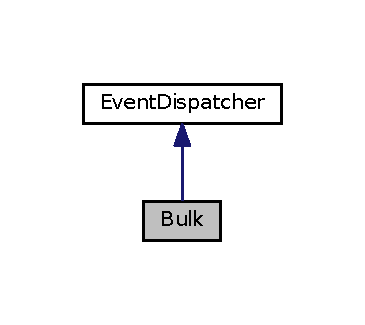
\includegraphics[width=175pt]{class_bulk__inherit__graph}
\end{center}
\end{figure}


Collaboration diagram for Bulk\+:
\nopagebreak
\begin{figure}[H]
\begin{center}
\leavevmode
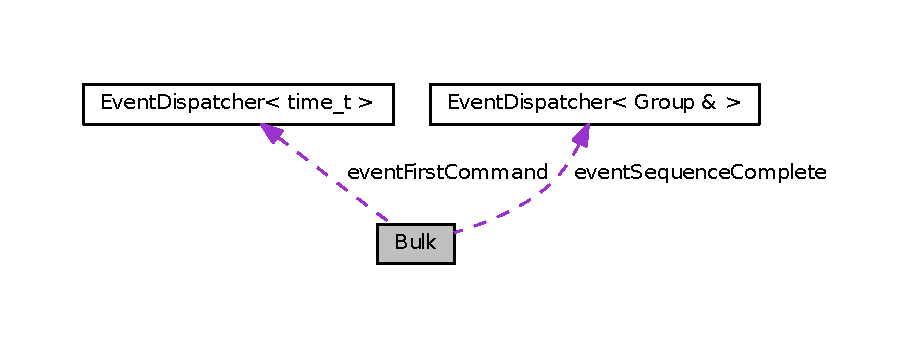
\includegraphics[width=175pt]{class_bulk__coll__graph}
\end{center}
\end{figure}
\subsection*{Public Member Functions}
\begin{DoxyCompactItemize}
\item 
\hyperlink{class_bulk_a3cb233a46de98d8111b7ae7606ba1460}{Bulk} (int \hyperlink{class_bulk_ac4c14e391ab0654fc1a2b6aea0b77410}{command\+Buf\+Count})
\item 
{\footnotesize template$<$typename T $>$ }\\void \hyperlink{class_bulk_ab420aeb70efbd54b1a7975c18da12c8f}{Set\+State} ()
\item 
std\+::shared\+\_\+ptr$<$ \hyperlink{class_i_interpreter_state}{I\+Interpreter\+State} $>$ \hyperlink{class_bulk_aa210e457c6f020835bde3bb67e0cfce3}{Get\+State} ()
\item 
void \hyperlink{class_bulk_a1be5c7493701769d6f95f1b37d94b752}{Run} ()
\end{DoxyCompactItemize}
\subsection*{Public Attributes}
\begin{DoxyCompactItemize}
\item 
int \hyperlink{class_bulk_ac4c14e391ab0654fc1a2b6aea0b77410}{command\+Buf\+Count}
\end{DoxyCompactItemize}


\subsection{Constructor \& Destructor Documentation}
\index{Bulk@{Bulk}!Bulk@{Bulk}}
\index{Bulk@{Bulk}!Bulk@{Bulk}}
\subsubsection[{\texorpdfstring{Bulk(int command\+Buf\+Count)}{Bulk(int commandBufCount)}}]{\setlength{\rightskip}{0pt plus 5cm}Bulk\+::\+Bulk (
\begin{DoxyParamCaption}
\item[{int}]{command\+Buf\+Count}
\end{DoxyParamCaption}
)\hspace{0.3cm}{\ttfamily [inline]}}\hypertarget{class_bulk_a3cb233a46de98d8111b7ae7606ba1460}{}\label{class_bulk_a3cb233a46de98d8111b7ae7606ba1460}


\subsection{Member Function Documentation}
\index{Bulk@{Bulk}!Get\+State@{Get\+State}}
\index{Get\+State@{Get\+State}!Bulk@{Bulk}}
\subsubsection[{\texorpdfstring{Get\+State()}{GetState()}}]{\setlength{\rightskip}{0pt plus 5cm}std\+::shared\+\_\+ptr$<${\bf I\+Interpreter\+State}$>$ Bulk\+::\+Get\+State (
\begin{DoxyParamCaption}
{}
\end{DoxyParamCaption}
)\hspace{0.3cm}{\ttfamily [inline]}}\hypertarget{class_bulk_aa210e457c6f020835bde3bb67e0cfce3}{}\label{class_bulk_aa210e457c6f020835bde3bb67e0cfce3}
\index{Bulk@{Bulk}!Run@{Run}}
\index{Run@{Run}!Bulk@{Bulk}}
\subsubsection[{\texorpdfstring{Run()}{Run()}}]{\setlength{\rightskip}{0pt plus 5cm}void Bulk\+::\+Run (
\begin{DoxyParamCaption}
{}
\end{DoxyParamCaption}
)\hspace{0.3cm}{\ttfamily [inline]}}\hypertarget{class_bulk_a1be5c7493701769d6f95f1b37d94b752}{}\label{class_bulk_a1be5c7493701769d6f95f1b37d94b752}
\index{Bulk@{Bulk}!Set\+State@{Set\+State}}
\index{Set\+State@{Set\+State}!Bulk@{Bulk}}
\subsubsection[{\texorpdfstring{Set\+State()}{SetState()}}]{\setlength{\rightskip}{0pt plus 5cm}template$<$typename T $>$ void Bulk\+::\+Set\+State (
\begin{DoxyParamCaption}
{}
\end{DoxyParamCaption}
)\hspace{0.3cm}{\ttfamily [inline]}}\hypertarget{class_bulk_ab420aeb70efbd54b1a7975c18da12c8f}{}\label{class_bulk_ab420aeb70efbd54b1a7975c18da12c8f}


\subsection{Member Data Documentation}
\index{Bulk@{Bulk}!command\+Buf\+Count@{command\+Buf\+Count}}
\index{command\+Buf\+Count@{command\+Buf\+Count}!Bulk@{Bulk}}
\subsubsection[{\texorpdfstring{command\+Buf\+Count}{commandBufCount}}]{\setlength{\rightskip}{0pt plus 5cm}int Bulk\+::command\+Buf\+Count}\hypertarget{class_bulk_ac4c14e391ab0654fc1a2b6aea0b77410}{}\label{class_bulk_ac4c14e391ab0654fc1a2b6aea0b77410}


The documentation for this class was generated from the following file\+:\begin{DoxyCompactItemize}
\item 
src/\hyperlink{_bulk_8h}{Bulk.\+h}\end{DoxyCompactItemize}

\hypertarget{struct_command}{}\section{Command Struct Reference}
\label{struct_command}\index{Command@{Command}}


{\ttfamily \#include $<$I\+Interpreter\+State.\+h$>$}



Inheritance diagram for Command\+:
\nopagebreak
\begin{figure}[H]
\begin{center}
\leavevmode
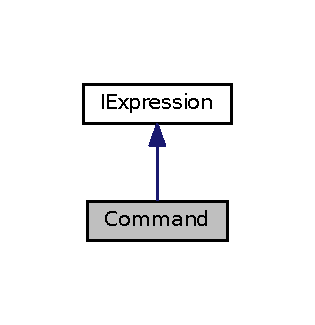
\includegraphics[width=151pt]{struct_command__inherit__graph}
\end{center}
\end{figure}


Collaboration diagram for Command\+:
\nopagebreak
\begin{figure}[H]
\begin{center}
\leavevmode
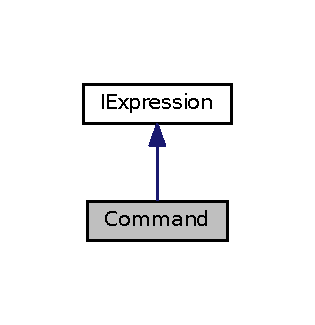
\includegraphics[width=151pt]{struct_command__coll__graph}
\end{center}
\end{figure}
\subsection*{Public Member Functions}
\begin{DoxyCompactItemize}
\item 
virtual \hyperlink{struct_command_ae4fd05a91d2e11794bd6427aa37b8c77}{operator std\+::string} () const override
\end{DoxyCompactItemize}
\subsection*{Public Attributes}
\begin{DoxyCompactItemize}
\item 
std\+::string \hyperlink{struct_command_a311f7e5b9aea6720e62c2ccb8a835eb7}{value}
\end{DoxyCompactItemize}


\subsection{Member Function Documentation}
\index{Command@{Command}!operator std\+::string@{operator std\+::string}}
\index{operator std\+::string@{operator std\+::string}!Command@{Command}}
\subsubsection[{\texorpdfstring{operator std\+::string() const override}{operator std::string() const override}}]{\setlength{\rightskip}{0pt plus 5cm}virtual Command\+::operator std\+::string (
\begin{DoxyParamCaption}
{}
\end{DoxyParamCaption}
) const\hspace{0.3cm}{\ttfamily [inline]}, {\ttfamily [override]}, {\ttfamily [virtual]}}\hypertarget{struct_command_ae4fd05a91d2e11794bd6427aa37b8c77}{}\label{struct_command_ae4fd05a91d2e11794bd6427aa37b8c77}


Implements \hyperlink{struct_i_expression_af8657bb1d333c4a3f3b97b449725bc9b}{I\+Expression}.



\subsection{Member Data Documentation}
\index{Command@{Command}!value@{value}}
\index{value@{value}!Command@{Command}}
\subsubsection[{\texorpdfstring{value}{value}}]{\setlength{\rightskip}{0pt plus 5cm}std\+::string Command\+::value}\hypertarget{struct_command_a311f7e5b9aea6720e62c2ccb8a835eb7}{}\label{struct_command_a311f7e5b9aea6720e62c2ccb8a835eb7}


The documentation for this struct was generated from the following file\+:\begin{DoxyCompactItemize}
\item 
src/\hyperlink{_i_interpreter_state_8h}{I\+Interpreter\+State.\+h}\end{DoxyCompactItemize}

\hypertarget{struct_console_logger}{}\section{Console\+Logger Struct Reference}
\label{struct_console_logger}\index{Console\+Logger@{Console\+Logger}}


{\ttfamily \#include $<$Console\+Logger.\+h$>$}

\subsection*{Public Member Functions}
\begin{DoxyCompactItemize}
\item 
void \hyperlink{struct_console_logger_a64169cc3b9f8a861dc874a6a174fd2e8}{Log} (std\+::string message)
\end{DoxyCompactItemize}


\subsection{Member Function Documentation}
\index{Console\+Logger@{Console\+Logger}!Log@{Log}}
\index{Log@{Log}!Console\+Logger@{Console\+Logger}}
\subsubsection[{\texorpdfstring{Log(std\+::string message)}{Log(std::string message)}}]{\setlength{\rightskip}{0pt plus 5cm}void Console\+Logger\+::\+Log (
\begin{DoxyParamCaption}
\item[{std\+::string}]{message}
\end{DoxyParamCaption}
)\hspace{0.3cm}{\ttfamily [inline]}}\hypertarget{struct_console_logger_a64169cc3b9f8a861dc874a6a174fd2e8}{}\label{struct_console_logger_a64169cc3b9f8a861dc874a6a174fd2e8}


The documentation for this struct was generated from the following file\+:\begin{DoxyCompactItemize}
\item 
src/log/\hyperlink{_console_logger_8h}{Console\+Logger.\+h}\end{DoxyCompactItemize}

\hypertarget{class_event_dispatcher}{}\section{Event\+Dispatcher$<$ Args $>$ Class Template Reference}
\label{class_event_dispatcher}\index{Event\+Dispatcher$<$ Args $>$@{Event\+Dispatcher$<$ Args $>$}}


{\ttfamily \#include $<$Event\+Dispatcher.\+h$>$}

\subsection*{Public Member Functions}
\begin{DoxyCompactItemize}
\item 
void \hyperlink{class_event_dispatcher_ac2faff743f86cad86215acd473f68c92}{Subscribe} (handler\+\_\+type \&\&handler)
\item 
void \hyperlink{class_event_dispatcher_ac696d0bc5b66ee4f3a13c469e8fc7975}{Unsubscribe\+All} ()
\item 
void \hyperlink{class_event_dispatcher_a6dfe75d89d1692665861bfd0e908c75e}{Dispatch} (Args...\+args)
\end{DoxyCompactItemize}


\subsection{Member Function Documentation}
\index{Event\+Dispatcher@{Event\+Dispatcher}!Dispatch@{Dispatch}}
\index{Dispatch@{Dispatch}!Event\+Dispatcher@{Event\+Dispatcher}}
\subsubsection[{\texorpdfstring{Dispatch(\+Args...\+args)}{Dispatch(Args...args)}}]{\setlength{\rightskip}{0pt plus 5cm}template$<$typename... Args$>$ void {\bf Event\+Dispatcher}$<$ Args $>$\+::Dispatch (
\begin{DoxyParamCaption}
\item[{Args...}]{args}
\end{DoxyParamCaption}
)\hspace{0.3cm}{\ttfamily [inline]}}\hypertarget{class_event_dispatcher_a6dfe75d89d1692665861bfd0e908c75e}{}\label{class_event_dispatcher_a6dfe75d89d1692665861bfd0e908c75e}
\index{Event\+Dispatcher@{Event\+Dispatcher}!Subscribe@{Subscribe}}
\index{Subscribe@{Subscribe}!Event\+Dispatcher@{Event\+Dispatcher}}
\subsubsection[{\texorpdfstring{Subscribe(handler\+\_\+type \&\&handler)}{Subscribe(handler_type &&handler)}}]{\setlength{\rightskip}{0pt plus 5cm}template$<$typename... Args$>$ void {\bf Event\+Dispatcher}$<$ Args $>$\+::Subscribe (
\begin{DoxyParamCaption}
\item[{handler\+\_\+type \&\&}]{handler}
\end{DoxyParamCaption}
)\hspace{0.3cm}{\ttfamily [inline]}}\hypertarget{class_event_dispatcher_ac2faff743f86cad86215acd473f68c92}{}\label{class_event_dispatcher_ac2faff743f86cad86215acd473f68c92}
\index{Event\+Dispatcher@{Event\+Dispatcher}!Unsubscribe\+All@{Unsubscribe\+All}}
\index{Unsubscribe\+All@{Unsubscribe\+All}!Event\+Dispatcher@{Event\+Dispatcher}}
\subsubsection[{\texorpdfstring{Unsubscribe\+All()}{UnsubscribeAll()}}]{\setlength{\rightskip}{0pt plus 5cm}template$<$typename... Args$>$ void {\bf Event\+Dispatcher}$<$ Args $>$\+::Unsubscribe\+All (
\begin{DoxyParamCaption}
{}
\end{DoxyParamCaption}
)\hspace{0.3cm}{\ttfamily [inline]}}\hypertarget{class_event_dispatcher_ac696d0bc5b66ee4f3a13c469e8fc7975}{}\label{class_event_dispatcher_ac696d0bc5b66ee4f3a13c469e8fc7975}


The documentation for this class was generated from the following file\+:\begin{DoxyCompactItemize}
\item 
src/events/\hyperlink{_event_dispatcher_8h}{Event\+Dispatcher.\+h}\end{DoxyCompactItemize}

\hypertarget{struct_file_logger}{}\section{File\+Logger Struct Reference}
\label{struct_file_logger}\index{File\+Logger@{File\+Logger}}


{\ttfamily \#include $<$File\+Logger.\+h$>$}

\subsection*{Public Member Functions}
\begin{DoxyCompactItemize}
\item 
void \hyperlink{struct_file_logger_a9f9d1f28631a59331a8922aeb67c124e}{Prepare\+Filename} (std\+::string file\+Name)
\item 
void \hyperlink{struct_file_logger_ad315ff83f838f680c83c22533cd63a26}{Log} (std\+::string message)
\end{DoxyCompactItemize}


\subsection{Member Function Documentation}
\index{File\+Logger@{File\+Logger}!Log@{Log}}
\index{Log@{Log}!File\+Logger@{File\+Logger}}
\subsubsection[{\texorpdfstring{Log(std\+::string message)}{Log(std::string message)}}]{\setlength{\rightskip}{0pt plus 5cm}void File\+Logger\+::\+Log (
\begin{DoxyParamCaption}
\item[{std\+::string}]{message}
\end{DoxyParamCaption}
)\hspace{0.3cm}{\ttfamily [inline]}}\hypertarget{struct_file_logger_ad315ff83f838f680c83c22533cd63a26}{}\label{struct_file_logger_ad315ff83f838f680c83c22533cd63a26}
\index{File\+Logger@{File\+Logger}!Prepare\+Filename@{Prepare\+Filename}}
\index{Prepare\+Filename@{Prepare\+Filename}!File\+Logger@{File\+Logger}}
\subsubsection[{\texorpdfstring{Prepare\+Filename(std\+::string file\+Name)}{PrepareFilename(std::string fileName)}}]{\setlength{\rightskip}{0pt plus 5cm}void File\+Logger\+::\+Prepare\+Filename (
\begin{DoxyParamCaption}
\item[{std\+::string}]{file\+Name}
\end{DoxyParamCaption}
)\hspace{0.3cm}{\ttfamily [inline]}}\hypertarget{struct_file_logger_a9f9d1f28631a59331a8922aeb67c124e}{}\label{struct_file_logger_a9f9d1f28631a59331a8922aeb67c124e}


The documentation for this struct was generated from the following file\+:\begin{DoxyCompactItemize}
\item 
src/log/\hyperlink{_file_logger_8h}{File\+Logger.\+h}\end{DoxyCompactItemize}

\hypertarget{struct_group}{}\section{Group Struct Reference}
\label{struct_group}\index{Group@{Group}}


{\ttfamily \#include $<$I\+Interpreter\+State.\+h$>$}



Inheritance diagram for Group\+:
\nopagebreak
\begin{figure}[H]
\begin{center}
\leavevmode
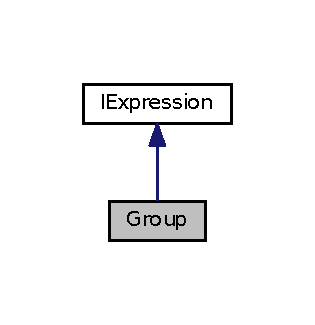
\includegraphics[width=151pt]{struct_group__inherit__graph}
\end{center}
\end{figure}


Collaboration diagram for Group\+:
\nopagebreak
\begin{figure}[H]
\begin{center}
\leavevmode
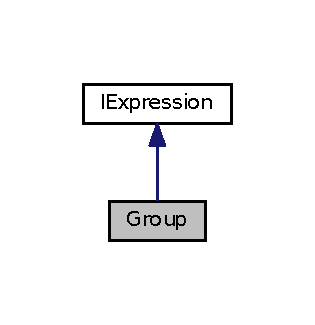
\includegraphics[width=151pt]{struct_group__coll__graph}
\end{center}
\end{figure}
\subsection*{Public Member Functions}
\begin{DoxyCompactItemize}
\item 
virtual \hyperlink{struct_group_a0ae2d99c278c335a0cc1a892c1a6eeb4}{operator std\+::string} () const override
\end{DoxyCompactItemize}
\subsection*{Public Attributes}
\begin{DoxyCompactItemize}
\item 
std\+::shared\+\_\+ptr$<$ \hyperlink{struct_group}{Group} $>$ \hyperlink{struct_group_a97509613c8c410bb6a3c281b102a1532}{parent}
\item 
std\+::vector$<$ std\+::shared\+\_\+ptr$<$ \hyperlink{struct_i_expression}{I\+Expression} $>$ $>$ \hyperlink{struct_group_a80ff87ea6dcbe39444fe0ac267819aec}{expressions}
\end{DoxyCompactItemize}


\subsection{Member Function Documentation}
\index{Group@{Group}!operator std\+::string@{operator std\+::string}}
\index{operator std\+::string@{operator std\+::string}!Group@{Group}}
\subsubsection[{\texorpdfstring{operator std\+::string() const override}{operator std::string() const override}}]{\setlength{\rightskip}{0pt plus 5cm}virtual Group\+::operator std\+::string (
\begin{DoxyParamCaption}
{}
\end{DoxyParamCaption}
) const\hspace{0.3cm}{\ttfamily [inline]}, {\ttfamily [override]}, {\ttfamily [virtual]}}\hypertarget{struct_group_a0ae2d99c278c335a0cc1a892c1a6eeb4}{}\label{struct_group_a0ae2d99c278c335a0cc1a892c1a6eeb4}


Implements \hyperlink{struct_i_expression_af8657bb1d333c4a3f3b97b449725bc9b}{I\+Expression}.



\subsection{Member Data Documentation}
\index{Group@{Group}!expressions@{expressions}}
\index{expressions@{expressions}!Group@{Group}}
\subsubsection[{\texorpdfstring{expressions}{expressions}}]{\setlength{\rightskip}{0pt plus 5cm}std\+::vector$<$std\+::shared\+\_\+ptr$<${\bf I\+Expression}$>$ $>$ Group\+::expressions}\hypertarget{struct_group_a80ff87ea6dcbe39444fe0ac267819aec}{}\label{struct_group_a80ff87ea6dcbe39444fe0ac267819aec}
\index{Group@{Group}!parent@{parent}}
\index{parent@{parent}!Group@{Group}}
\subsubsection[{\texorpdfstring{parent}{parent}}]{\setlength{\rightskip}{0pt plus 5cm}std\+::shared\+\_\+ptr$<${\bf Group}$>$ Group\+::parent}\hypertarget{struct_group_a97509613c8c410bb6a3c281b102a1532}{}\label{struct_group_a97509613c8c410bb6a3c281b102a1532}


The documentation for this struct was generated from the following file\+:\begin{DoxyCompactItemize}
\item 
src/\hyperlink{_i_interpreter_state_8h}{I\+Interpreter\+State.\+h}\end{DoxyCompactItemize}

\hypertarget{struct_i_expression}{}\section{I\+Expression Struct Reference}
\label{struct_i_expression}\index{I\+Expression@{I\+Expression}}


{\ttfamily \#include $<$I\+Interpreter\+State.\+h$>$}



Inheritance diagram for I\+Expression\+:
\nopagebreak
\begin{figure}[H]
\begin{center}
\leavevmode
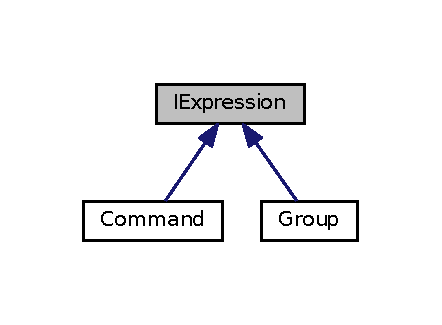
\includegraphics[width=212pt]{struct_i_expression__inherit__graph}
\end{center}
\end{figure}
\subsection*{Public Member Functions}
\begin{DoxyCompactItemize}
\item 
virtual \hyperlink{struct_i_expression_af9783c70a37f2472d1a1d8baa484fd85}{$\sim$\+I\+Expression} ()
\item 
virtual \hyperlink{struct_i_expression_af8657bb1d333c4a3f3b97b449725bc9b}{operator std\+::string} () const =0
\end{DoxyCompactItemize}


\subsection{Constructor \& Destructor Documentation}
\index{I\+Expression@{I\+Expression}!````~I\+Expression@{$\sim$\+I\+Expression}}
\index{````~I\+Expression@{$\sim$\+I\+Expression}!I\+Expression@{I\+Expression}}
\subsubsection[{\texorpdfstring{$\sim$\+I\+Expression()}{~IExpression()}}]{\setlength{\rightskip}{0pt plus 5cm}virtual I\+Expression\+::$\sim$\+I\+Expression (
\begin{DoxyParamCaption}
{}
\end{DoxyParamCaption}
)\hspace{0.3cm}{\ttfamily [inline]}, {\ttfamily [virtual]}}\hypertarget{struct_i_expression_af9783c70a37f2472d1a1d8baa484fd85}{}\label{struct_i_expression_af9783c70a37f2472d1a1d8baa484fd85}


\subsection{Member Function Documentation}
\index{I\+Expression@{I\+Expression}!operator std\+::string@{operator std\+::string}}
\index{operator std\+::string@{operator std\+::string}!I\+Expression@{I\+Expression}}
\subsubsection[{\texorpdfstring{operator std\+::string() const =0}{operator std::string() const =0}}]{\setlength{\rightskip}{0pt plus 5cm}virtual I\+Expression\+::operator std\+::string (
\begin{DoxyParamCaption}
{}
\end{DoxyParamCaption}
) const\hspace{0.3cm}{\ttfamily [pure virtual]}}\hypertarget{struct_i_expression_af8657bb1d333c4a3f3b97b449725bc9b}{}\label{struct_i_expression_af8657bb1d333c4a3f3b97b449725bc9b}


Implemented in \hyperlink{struct_group_a0ae2d99c278c335a0cc1a892c1a6eeb4}{Group}, and \hyperlink{struct_command_ae4fd05a91d2e11794bd6427aa37b8c77}{Command}.



The documentation for this struct was generated from the following file\+:\begin{DoxyCompactItemize}
\item 
src/\hyperlink{_i_interpreter_state_8h}{I\+Interpreter\+State.\+h}\end{DoxyCompactItemize}

\hypertarget{class_i_interpreter_state}{}\section{I\+Interpreter\+State Class Reference}
\label{class_i_interpreter_state}\index{I\+Interpreter\+State@{I\+Interpreter\+State}}


{\ttfamily \#include $<$I\+Interpreter\+State.\+h$>$}



Inheritance diagram for I\+Interpreter\+State\+:
\nopagebreak
\begin{figure}[H]
\begin{center}
\leavevmode
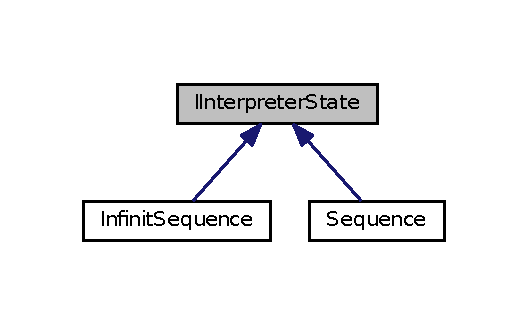
\includegraphics[width=254pt]{class_i_interpreter_state__inherit__graph}
\end{center}
\end{figure}


Collaboration diagram for I\+Interpreter\+State\+:
\nopagebreak
\begin{figure}[H]
\begin{center}
\leavevmode
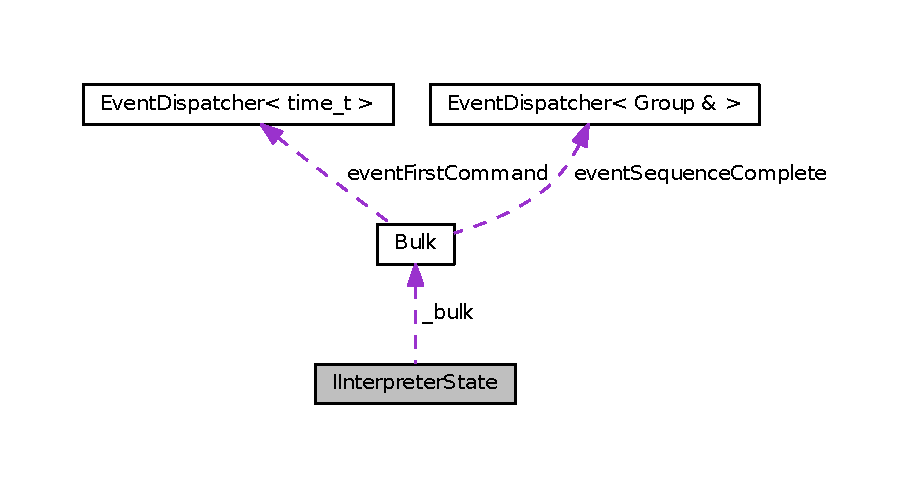
\includegraphics[width=350pt]{class_i_interpreter_state__coll__graph}
\end{center}
\end{figure}
\subsection*{Public Member Functions}
\begin{DoxyCompactItemize}
\item 
\hyperlink{class_i_interpreter_state_a0f1558e06d52278321e94d64f7f5e2d9}{I\+Interpreter\+State} (\hyperlink{class_bulk}{Bulk} \&bulk)
\item 
virtual \hyperlink{class_i_interpreter_state_a12d0d93f030ee75d63cffcf684e1062d}{$\sim$\+I\+Interpreter\+State} ()
\item 
virtual void \hyperlink{class_i_interpreter_state_a4a8559db87100cc214e544d274ee4174}{Initialize} ()
\item 
virtual void \hyperlink{class_i_interpreter_state_ac178373a2622323811db25b6a118aef4}{Exec} (std\+::string ctx)=0
\item 
virtual void \hyperlink{class_i_interpreter_state_abdc7f5e834aa48047959152b4a090c08}{Finalize} ()
\end{DoxyCompactItemize}
\subsection*{Protected Attributes}
\begin{DoxyCompactItemize}
\item 
\hyperlink{class_bulk}{Bulk} \& \hyperlink{class_i_interpreter_state_a3c0b3f4d608c3d79fa38611ff50ce030}{\+\_\+bulk}
\end{DoxyCompactItemize}


\subsection{Constructor \& Destructor Documentation}
\index{I\+Interpreter\+State@{I\+Interpreter\+State}!I\+Interpreter\+State@{I\+Interpreter\+State}}
\index{I\+Interpreter\+State@{I\+Interpreter\+State}!I\+Interpreter\+State@{I\+Interpreter\+State}}
\subsubsection[{\texorpdfstring{I\+Interpreter\+State(\+Bulk \&bulk)}{IInterpreterState(Bulk &bulk)}}]{\setlength{\rightskip}{0pt plus 5cm}I\+Interpreter\+State\+::\+I\+Interpreter\+State (
\begin{DoxyParamCaption}
\item[{{\bf Bulk} \&}]{bulk}
\end{DoxyParamCaption}
)\hspace{0.3cm}{\ttfamily [inline]}}\hypertarget{class_i_interpreter_state_a0f1558e06d52278321e94d64f7f5e2d9}{}\label{class_i_interpreter_state_a0f1558e06d52278321e94d64f7f5e2d9}
\index{I\+Interpreter\+State@{I\+Interpreter\+State}!````~I\+Interpreter\+State@{$\sim$\+I\+Interpreter\+State}}
\index{````~I\+Interpreter\+State@{$\sim$\+I\+Interpreter\+State}!I\+Interpreter\+State@{I\+Interpreter\+State}}
\subsubsection[{\texorpdfstring{$\sim$\+I\+Interpreter\+State()}{~IInterpreterState()}}]{\setlength{\rightskip}{0pt plus 5cm}virtual I\+Interpreter\+State\+::$\sim$\+I\+Interpreter\+State (
\begin{DoxyParamCaption}
{}
\end{DoxyParamCaption}
)\hspace{0.3cm}{\ttfamily [inline]}, {\ttfamily [virtual]}}\hypertarget{class_i_interpreter_state_a12d0d93f030ee75d63cffcf684e1062d}{}\label{class_i_interpreter_state_a12d0d93f030ee75d63cffcf684e1062d}


\subsection{Member Function Documentation}
\index{I\+Interpreter\+State@{I\+Interpreter\+State}!Exec@{Exec}}
\index{Exec@{Exec}!I\+Interpreter\+State@{I\+Interpreter\+State}}
\subsubsection[{\texorpdfstring{Exec(std\+::string ctx)=0}{Exec(std::string ctx)=0}}]{\setlength{\rightskip}{0pt plus 5cm}virtual void I\+Interpreter\+State\+::\+Exec (
\begin{DoxyParamCaption}
\item[{std\+::string}]{ctx}
\end{DoxyParamCaption}
)\hspace{0.3cm}{\ttfamily [pure virtual]}}\hypertarget{class_i_interpreter_state_ac178373a2622323811db25b6a118aef4}{}\label{class_i_interpreter_state_ac178373a2622323811db25b6a118aef4}


Implemented in \hyperlink{class_infinit_sequence_ab12080f4b10b97c2a5e457746a7301c1}{Infinit\+Sequence}, and \hyperlink{class_sequence_ab87fad512892328443acaadcd9c10379}{Sequence}.

\index{I\+Interpreter\+State@{I\+Interpreter\+State}!Finalize@{Finalize}}
\index{Finalize@{Finalize}!I\+Interpreter\+State@{I\+Interpreter\+State}}
\subsubsection[{\texorpdfstring{Finalize()}{Finalize()}}]{\setlength{\rightskip}{0pt plus 5cm}virtual void I\+Interpreter\+State\+::\+Finalize (
\begin{DoxyParamCaption}
{}
\end{DoxyParamCaption}
)\hspace{0.3cm}{\ttfamily [inline]}, {\ttfamily [virtual]}}\hypertarget{class_i_interpreter_state_abdc7f5e834aa48047959152b4a090c08}{}\label{class_i_interpreter_state_abdc7f5e834aa48047959152b4a090c08}


Reimplemented in \hyperlink{class_sequence_a48787febf1f2bbaaedfc0a7b957e8822}{Sequence}, and \hyperlink{class_infinit_sequence_ab28b9e2f1106aabaa69a6dfbb716ea73}{Infinit\+Sequence}.

\index{I\+Interpreter\+State@{I\+Interpreter\+State}!Initialize@{Initialize}}
\index{Initialize@{Initialize}!I\+Interpreter\+State@{I\+Interpreter\+State}}
\subsubsection[{\texorpdfstring{Initialize()}{Initialize()}}]{\setlength{\rightskip}{0pt plus 5cm}virtual void I\+Interpreter\+State\+::\+Initialize (
\begin{DoxyParamCaption}
{}
\end{DoxyParamCaption}
)\hspace{0.3cm}{\ttfamily [inline]}, {\ttfamily [virtual]}}\hypertarget{class_i_interpreter_state_a4a8559db87100cc214e544d274ee4174}{}\label{class_i_interpreter_state_a4a8559db87100cc214e544d274ee4174}


Reimplemented in \hyperlink{class_sequence_a719a07060acf25ccdca5216af71eaed7}{Sequence}, and \hyperlink{class_infinit_sequence_a53f4ee00e5659bb61b6af8ab1bcc24a5}{Infinit\+Sequence}.



\subsection{Member Data Documentation}
\index{I\+Interpreter\+State@{I\+Interpreter\+State}!\+\_\+bulk@{\+\_\+bulk}}
\index{\+\_\+bulk@{\+\_\+bulk}!I\+Interpreter\+State@{I\+Interpreter\+State}}
\subsubsection[{\texorpdfstring{\+\_\+bulk}{_bulk}}]{\setlength{\rightskip}{0pt plus 5cm}{\bf Bulk}\& I\+Interpreter\+State\+::\+\_\+bulk\hspace{0.3cm}{\ttfamily [protected]}}\hypertarget{class_i_interpreter_state_a3c0b3f4d608c3d79fa38611ff50ce030}{}\label{class_i_interpreter_state_a3c0b3f4d608c3d79fa38611ff50ce030}


The documentation for this class was generated from the following file\+:\begin{DoxyCompactItemize}
\item 
src/\hyperlink{_i_interpreter_state_8h}{I\+Interpreter\+State.\+h}\end{DoxyCompactItemize}

\hypertarget{class_infinit_sequence}{}\section{Infinit\+Sequence Class Reference}
\label{class_infinit_sequence}\index{Infinit\+Sequence@{Infinit\+Sequence}}


{\ttfamily \#include $<$Infinit\+Sequence.\+h$>$}



Inheritance diagram for Infinit\+Sequence\+:
\nopagebreak
\begin{figure}[H]
\begin{center}
\leavevmode
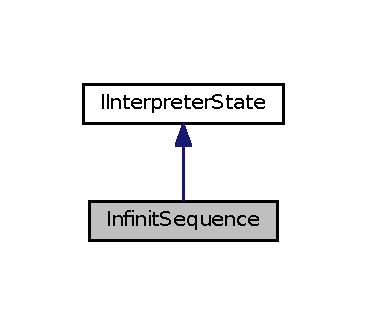
\includegraphics[width=176pt]{class_infinit_sequence__inherit__graph}
\end{center}
\end{figure}


Collaboration diagram for Infinit\+Sequence\+:
\nopagebreak
\begin{figure}[H]
\begin{center}
\leavevmode
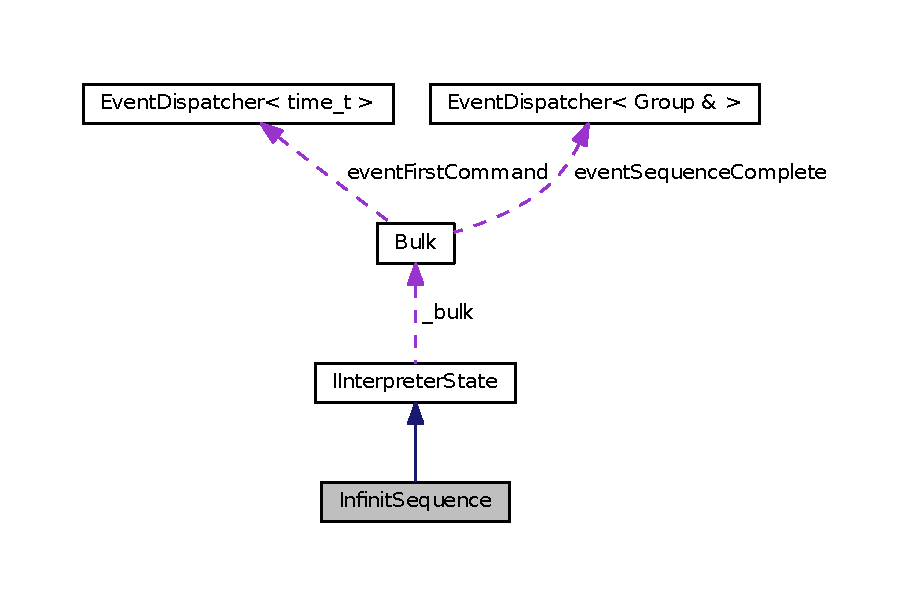
\includegraphics[width=176pt]{class_infinit_sequence__coll__graph}
\end{center}
\end{figure}
\subsection*{Public Member Functions}
\begin{DoxyCompactItemize}
\item 
\hyperlink{class_infinit_sequence_a7d326180468abe14bc3c3a89a02ae6b2}{Infinit\+Sequence} (\hyperlink{class_bulk}{Bulk} \&bulk)
\item 
virtual void \hyperlink{class_infinit_sequence_a53f4ee00e5659bb61b6af8ab1bcc24a5}{Initialize} () override
\item 
virtual void \hyperlink{class_infinit_sequence_ab28b9e2f1106aabaa69a6dfbb716ea73}{Finalize} () override
\item 
virtual void \hyperlink{class_infinit_sequence_ab12080f4b10b97c2a5e457746a7301c1}{Exec} (std\+::string ctx) override
\end{DoxyCompactItemize}
\subsection*{Protected Attributes}
\begin{DoxyCompactItemize}
\item 
std\+::shared\+\_\+ptr$<$ \hyperlink{struct_group}{Group} $>$ \hyperlink{class_infinit_sequence_ababeabf069e6bd4d53be04d2962fe990}{\+\_\+root\+Group}
\item 
std\+::shared\+\_\+ptr$<$ \hyperlink{struct_group}{Group} $>$ \hyperlink{class_infinit_sequence_afd8d7da621ed72083b00d75297b7f992}{\+\_\+current\+Group}
\item 
bool \hyperlink{class_infinit_sequence_ae10e9c4c746b3b7bc01c1d196bc05aa2}{\+\_\+await\+First\+Command} = true
\end{DoxyCompactItemize}


\subsection{Constructor \& Destructor Documentation}
\index{Infinit\+Sequence@{Infinit\+Sequence}!Infinit\+Sequence@{Infinit\+Sequence}}
\index{Infinit\+Sequence@{Infinit\+Sequence}!Infinit\+Sequence@{Infinit\+Sequence}}
\subsubsection[{\texorpdfstring{Infinit\+Sequence(\+Bulk \&bulk)}{InfinitSequence(Bulk &bulk)}}]{\setlength{\rightskip}{0pt plus 5cm}Infinit\+Sequence\+::\+Infinit\+Sequence (
\begin{DoxyParamCaption}
\item[{{\bf Bulk} \&}]{bulk}
\end{DoxyParamCaption}
)}\hypertarget{class_infinit_sequence_a7d326180468abe14bc3c3a89a02ae6b2}{}\label{class_infinit_sequence_a7d326180468abe14bc3c3a89a02ae6b2}


\subsection{Member Function Documentation}
\index{Infinit\+Sequence@{Infinit\+Sequence}!Exec@{Exec}}
\index{Exec@{Exec}!Infinit\+Sequence@{Infinit\+Sequence}}
\subsubsection[{\texorpdfstring{Exec(std\+::string ctx) override}{Exec(std::string ctx) override}}]{\setlength{\rightskip}{0pt plus 5cm}void Infinit\+Sequence\+::\+Exec (
\begin{DoxyParamCaption}
\item[{std\+::string}]{ctx}
\end{DoxyParamCaption}
)\hspace{0.3cm}{\ttfamily [override]}, {\ttfamily [virtual]}}\hypertarget{class_infinit_sequence_ab12080f4b10b97c2a5e457746a7301c1}{}\label{class_infinit_sequence_ab12080f4b10b97c2a5e457746a7301c1}


Implements \hyperlink{class_i_interpreter_state_ac178373a2622323811db25b6a118aef4}{I\+Interpreter\+State}.

\index{Infinit\+Sequence@{Infinit\+Sequence}!Finalize@{Finalize}}
\index{Finalize@{Finalize}!Infinit\+Sequence@{Infinit\+Sequence}}
\subsubsection[{\texorpdfstring{Finalize() override}{Finalize() override}}]{\setlength{\rightskip}{0pt plus 5cm}void Infinit\+Sequence\+::\+Finalize (
\begin{DoxyParamCaption}
{}
\end{DoxyParamCaption}
)\hspace{0.3cm}{\ttfamily [override]}, {\ttfamily [virtual]}}\hypertarget{class_infinit_sequence_ab28b9e2f1106aabaa69a6dfbb716ea73}{}\label{class_infinit_sequence_ab28b9e2f1106aabaa69a6dfbb716ea73}


Reimplemented from \hyperlink{class_i_interpreter_state_abdc7f5e834aa48047959152b4a090c08}{I\+Interpreter\+State}.

\index{Infinit\+Sequence@{Infinit\+Sequence}!Initialize@{Initialize}}
\index{Initialize@{Initialize}!Infinit\+Sequence@{Infinit\+Sequence}}
\subsubsection[{\texorpdfstring{Initialize() override}{Initialize() override}}]{\setlength{\rightskip}{0pt plus 5cm}void Infinit\+Sequence\+::\+Initialize (
\begin{DoxyParamCaption}
{}
\end{DoxyParamCaption}
)\hspace{0.3cm}{\ttfamily [override]}, {\ttfamily [virtual]}}\hypertarget{class_infinit_sequence_a53f4ee00e5659bb61b6af8ab1bcc24a5}{}\label{class_infinit_sequence_a53f4ee00e5659bb61b6af8ab1bcc24a5}


Reimplemented from \hyperlink{class_i_interpreter_state_a4a8559db87100cc214e544d274ee4174}{I\+Interpreter\+State}.



\subsection{Member Data Documentation}
\index{Infinit\+Sequence@{Infinit\+Sequence}!\+\_\+await\+First\+Command@{\+\_\+await\+First\+Command}}
\index{\+\_\+await\+First\+Command@{\+\_\+await\+First\+Command}!Infinit\+Sequence@{Infinit\+Sequence}}
\subsubsection[{\texorpdfstring{\+\_\+await\+First\+Command}{_awaitFirstCommand}}]{\setlength{\rightskip}{0pt plus 5cm}bool Infinit\+Sequence\+::\+\_\+await\+First\+Command = true\hspace{0.3cm}{\ttfamily [protected]}}\hypertarget{class_infinit_sequence_ae10e9c4c746b3b7bc01c1d196bc05aa2}{}\label{class_infinit_sequence_ae10e9c4c746b3b7bc01c1d196bc05aa2}
\index{Infinit\+Sequence@{Infinit\+Sequence}!\+\_\+current\+Group@{\+\_\+current\+Group}}
\index{\+\_\+current\+Group@{\+\_\+current\+Group}!Infinit\+Sequence@{Infinit\+Sequence}}
\subsubsection[{\texorpdfstring{\+\_\+current\+Group}{_currentGroup}}]{\setlength{\rightskip}{0pt plus 5cm}std\+::shared\+\_\+ptr$<${\bf Group}$>$ Infinit\+Sequence\+::\+\_\+current\+Group\hspace{0.3cm}{\ttfamily [protected]}}\hypertarget{class_infinit_sequence_afd8d7da621ed72083b00d75297b7f992}{}\label{class_infinit_sequence_afd8d7da621ed72083b00d75297b7f992}
\index{Infinit\+Sequence@{Infinit\+Sequence}!\+\_\+root\+Group@{\+\_\+root\+Group}}
\index{\+\_\+root\+Group@{\+\_\+root\+Group}!Infinit\+Sequence@{Infinit\+Sequence}}
\subsubsection[{\texorpdfstring{\+\_\+root\+Group}{_rootGroup}}]{\setlength{\rightskip}{0pt plus 5cm}std\+::shared\+\_\+ptr$<${\bf Group}$>$ Infinit\+Sequence\+::\+\_\+root\+Group\hspace{0.3cm}{\ttfamily [protected]}}\hypertarget{class_infinit_sequence_ababeabf069e6bd4d53be04d2962fe990}{}\label{class_infinit_sequence_ababeabf069e6bd4d53be04d2962fe990}


The documentation for this class was generated from the following files\+:\begin{DoxyCompactItemize}
\item 
src/\hyperlink{_infinit_sequence_8h}{Infinit\+Sequence.\+h}\item 
src/\hyperlink{_infinit_sequence_8cpp}{Infinit\+Sequence.\+cpp}\end{DoxyCompactItemize}

\hypertarget{class_sequence}{}\section{Sequence Class Reference}
\label{class_sequence}\index{Sequence@{Sequence}}


{\ttfamily \#include $<$Sequence.\+h$>$}



Inheritance diagram for Sequence\+:
\nopagebreak
\begin{figure}[H]
\begin{center}
\leavevmode
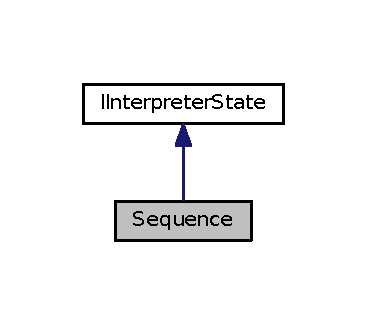
\includegraphics[width=176pt]{class_sequence__inherit__graph}
\end{center}
\end{figure}


Collaboration diagram for Sequence\+:
\nopagebreak
\begin{figure}[H]
\begin{center}
\leavevmode
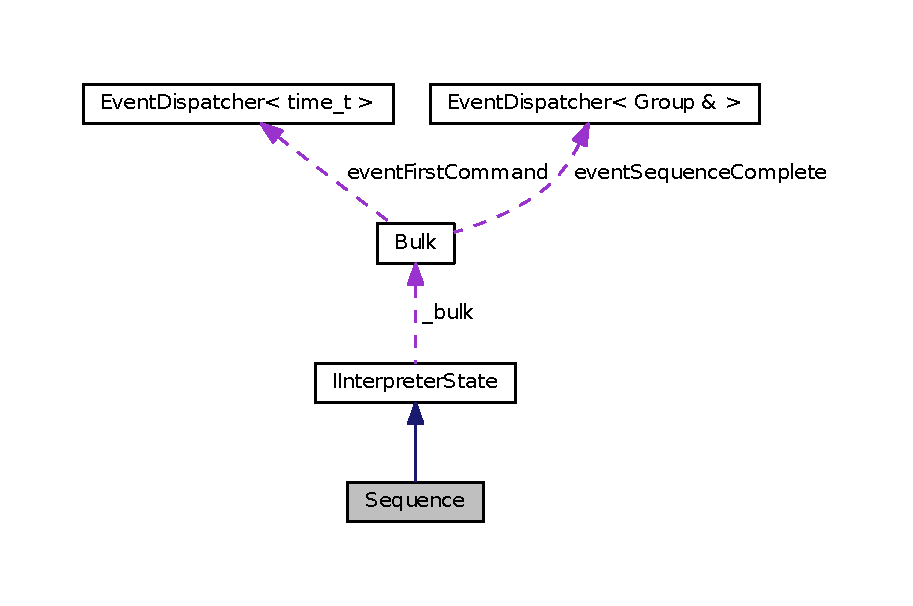
\includegraphics[width=176pt]{class_sequence__coll__graph}
\end{center}
\end{figure}
\subsection*{Public Member Functions}
\begin{DoxyCompactItemize}
\item 
\hyperlink{class_sequence_a6f8507db56fc8371afc94e3f735e6fc4}{Sequence} (\hyperlink{class_bulk}{Bulk} \&bulk)
\item 
virtual void \hyperlink{class_sequence_ab87fad512892328443acaadcd9c10379}{Exec} (std\+::string ctx) override
\item 
virtual void \hyperlink{class_sequence_a719a07060acf25ccdca5216af71eaed7}{Initialize} () override
\item 
virtual void \hyperlink{class_sequence_a48787febf1f2bbaaedfc0a7b957e8822}{Finalize} () override
\end{DoxyCompactItemize}
\subsection*{Additional Inherited Members}


\subsection{Constructor \& Destructor Documentation}
\index{Sequence@{Sequence}!Sequence@{Sequence}}
\index{Sequence@{Sequence}!Sequence@{Sequence}}
\subsubsection[{\texorpdfstring{Sequence(\+Bulk \&bulk)}{Sequence(Bulk &bulk)}}]{\setlength{\rightskip}{0pt plus 5cm}Sequence\+::\+Sequence (
\begin{DoxyParamCaption}
\item[{{\bf Bulk} \&}]{bulk}
\end{DoxyParamCaption}
)}\hypertarget{class_sequence_a6f8507db56fc8371afc94e3f735e6fc4}{}\label{class_sequence_a6f8507db56fc8371afc94e3f735e6fc4}


\subsection{Member Function Documentation}
\index{Sequence@{Sequence}!Exec@{Exec}}
\index{Exec@{Exec}!Sequence@{Sequence}}
\subsubsection[{\texorpdfstring{Exec(std\+::string ctx) override}{Exec(std::string ctx) override}}]{\setlength{\rightskip}{0pt plus 5cm}void Sequence\+::\+Exec (
\begin{DoxyParamCaption}
\item[{std\+::string}]{ctx}
\end{DoxyParamCaption}
)\hspace{0.3cm}{\ttfamily [override]}, {\ttfamily [virtual]}}\hypertarget{class_sequence_ab87fad512892328443acaadcd9c10379}{}\label{class_sequence_ab87fad512892328443acaadcd9c10379}


Implements \hyperlink{class_i_interpreter_state_ac178373a2622323811db25b6a118aef4}{I\+Interpreter\+State}.

\index{Sequence@{Sequence}!Finalize@{Finalize}}
\index{Finalize@{Finalize}!Sequence@{Sequence}}
\subsubsection[{\texorpdfstring{Finalize() override}{Finalize() override}}]{\setlength{\rightskip}{0pt plus 5cm}void Sequence\+::\+Finalize (
\begin{DoxyParamCaption}
{}
\end{DoxyParamCaption}
)\hspace{0.3cm}{\ttfamily [override]}, {\ttfamily [virtual]}}\hypertarget{class_sequence_a48787febf1f2bbaaedfc0a7b957e8822}{}\label{class_sequence_a48787febf1f2bbaaedfc0a7b957e8822}


Reimplemented from \hyperlink{class_i_interpreter_state_abdc7f5e834aa48047959152b4a090c08}{I\+Interpreter\+State}.

\index{Sequence@{Sequence}!Initialize@{Initialize}}
\index{Initialize@{Initialize}!Sequence@{Sequence}}
\subsubsection[{\texorpdfstring{Initialize() override}{Initialize() override}}]{\setlength{\rightskip}{0pt plus 5cm}void Sequence\+::\+Initialize (
\begin{DoxyParamCaption}
{}
\end{DoxyParamCaption}
)\hspace{0.3cm}{\ttfamily [override]}, {\ttfamily [virtual]}}\hypertarget{class_sequence_a719a07060acf25ccdca5216af71eaed7}{}\label{class_sequence_a719a07060acf25ccdca5216af71eaed7}


Reimplemented from \hyperlink{class_i_interpreter_state_a4a8559db87100cc214e544d274ee4174}{I\+Interpreter\+State}.



The documentation for this class was generated from the following files\+:\begin{DoxyCompactItemize}
\item 
src/\hyperlink{_sequence_8h}{Sequence.\+h}\item 
src/\hyperlink{_sequence_8cpp}{Sequence.\+cpp}\end{DoxyCompactItemize}

\chapter{File Documentation}
\hypertarget{_bulk_8h}{}\section{src/\+Bulk.h File Reference}
\label{_bulk_8h}\index{src/\+Bulk.\+h@{src/\+Bulk.\+h}}
{\ttfamily \#include $<$iostream$>$}\\*
{\ttfamily \#include $<$vector$>$}\\*
{\ttfamily \#include $<$map$>$}\\*
{\ttfamily \#include $<$typeindex$>$}\\*
{\ttfamily \#include \char`\"{}I\+Interpreter\+State.\+h\char`\"{}}\\*
{\ttfamily \#include \char`\"{}Sequence.\+h\char`\"{}}\\*
{\ttfamily \#include \char`\"{}Infinit\+Sequence.\+h\char`\"{}}\\*
{\ttfamily \#include \char`\"{}events/\+Event\+Dispatcher.\+h\char`\"{}}\\*
Include dependency graph for Bulk.\+h\+:
\nopagebreak
\begin{figure}[H]
\begin{center}
\leavevmode
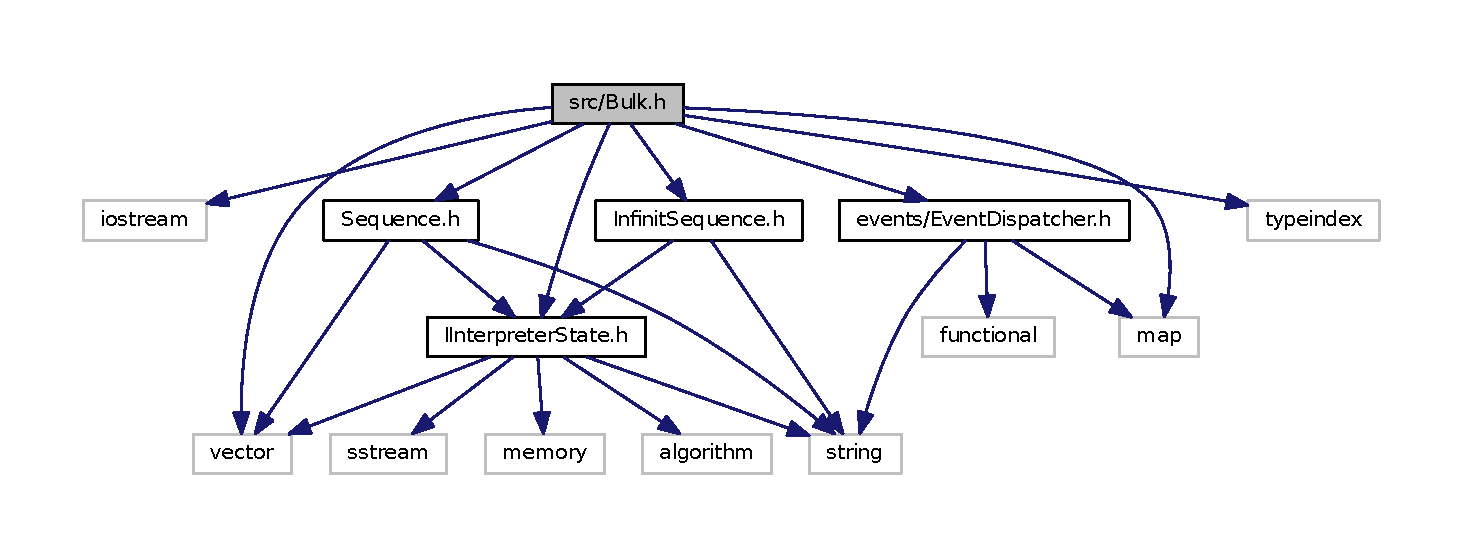
\includegraphics[width=350pt]{_bulk_8h__incl}
\end{center}
\end{figure}
This graph shows which files directly or indirectly include this file\+:
\nopagebreak
\begin{figure}[H]
\begin{center}
\leavevmode
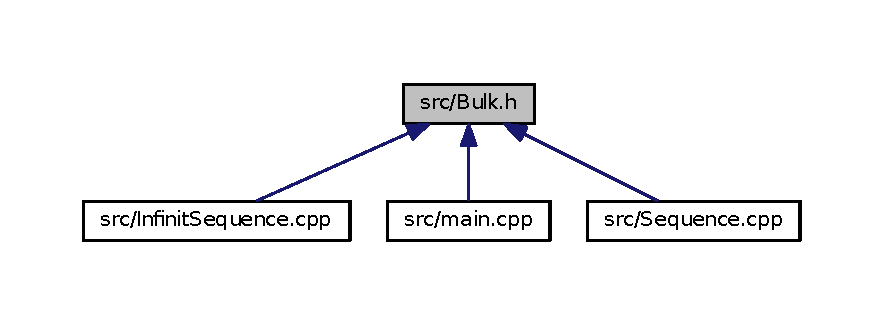
\includegraphics[width=350pt]{_bulk_8h__dep__incl}
\end{center}
\end{figure}
\subsection*{Classes}
\begin{DoxyCompactItemize}
\item 
class \hyperlink{class_bulk}{Bulk}
\end{DoxyCompactItemize}

\hypertarget{_event_dispatcher_8h}{}\section{src/events/\+Event\+Dispatcher.h File Reference}
\label{_event_dispatcher_8h}\index{src/events/\+Event\+Dispatcher.\+h@{src/events/\+Event\+Dispatcher.\+h}}
{\ttfamily \#include $<$string$>$}\\*
{\ttfamily \#include $<$functional$>$}\\*
{\ttfamily \#include $<$map$>$}\\*
Include dependency graph for Event\+Dispatcher.\+h\+:
\nopagebreak
\begin{figure}[H]
\begin{center}
\leavevmode
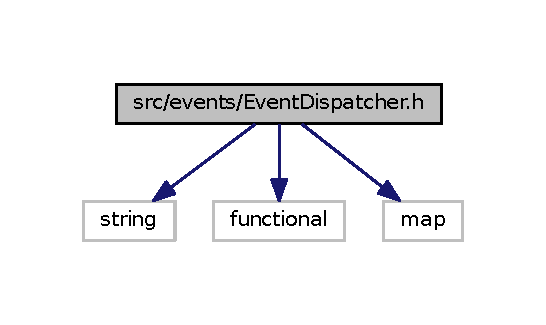
\includegraphics[width=262pt]{_event_dispatcher_8h__incl}
\end{center}
\end{figure}
This graph shows which files directly or indirectly include this file\+:
\nopagebreak
\begin{figure}[H]
\begin{center}
\leavevmode
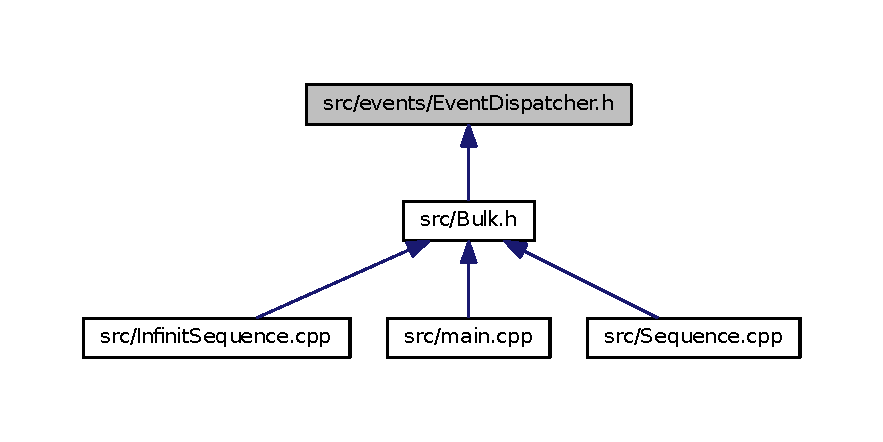
\includegraphics[width=350pt]{_event_dispatcher_8h__dep__incl}
\end{center}
\end{figure}
\subsection*{Classes}
\begin{DoxyCompactItemize}
\item 
class \hyperlink{class_event_dispatcher}{Event\+Dispatcher}
\end{DoxyCompactItemize}
\subsection*{Namespaces}
\begin{DoxyCompactItemize}
\item 
 \hyperlink{namespace_event}{Event}
\end{DoxyCompactItemize}

\hypertarget{_i_interpreter_state_8h}{}\section{src/\+I\+Interpreter\+State.h File Reference}
\label{_i_interpreter_state_8h}\index{src/\+I\+Interpreter\+State.\+h@{src/\+I\+Interpreter\+State.\+h}}
{\ttfamily \#include $<$utils/utils.\+h$>$}\\*
{\ttfamily \#include $<$string$>$}\\*
{\ttfamily \#include $<$vector$>$}\\*
{\ttfamily \#include $<$memory$>$}\\*
Include dependency graph for I\+Interpreter\+State.\+h\+:
\nopagebreak
\begin{figure}[H]
\begin{center}
\leavevmode
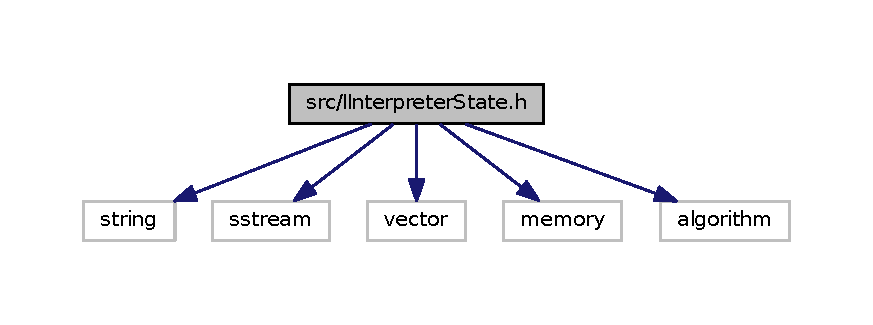
\includegraphics[width=350pt]{_i_interpreter_state_8h__incl}
\end{center}
\end{figure}
This graph shows which files directly or indirectly include this file\+:
\nopagebreak
\begin{figure}[H]
\begin{center}
\leavevmode
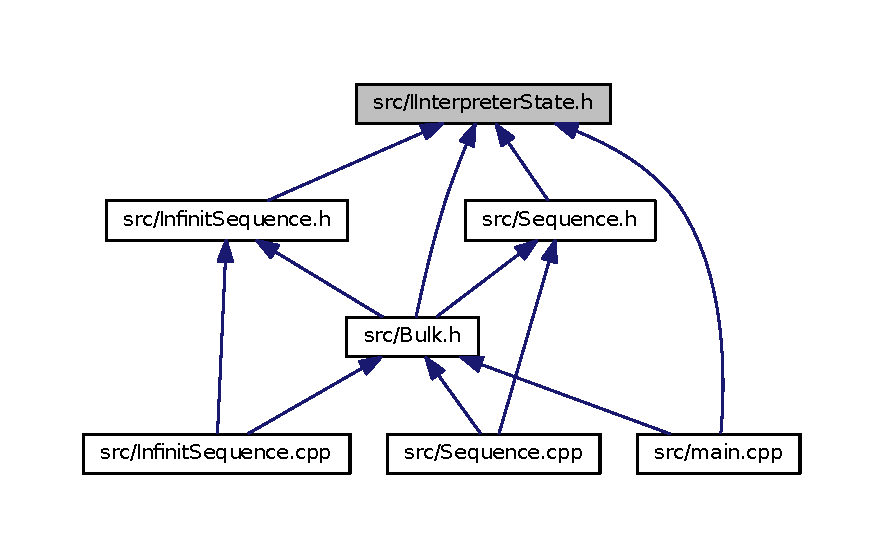
\includegraphics[width=350pt]{_i_interpreter_state_8h__dep__incl}
\end{center}
\end{figure}
\subsection*{Classes}
\begin{DoxyCompactItemize}
\item 
class \hyperlink{class_i_interpreter_state}{I\+Interpreter\+State}
\item 
struct \hyperlink{struct_i_expression}{I\+Expression}
\item 
struct \hyperlink{struct_command}{Command}
\item 
struct \hyperlink{struct_group}{Group}
\end{DoxyCompactItemize}

\hypertarget{_infinit_sequence_8cpp}{}\section{src/\+Infinit\+Sequence.cpp File Reference}
\label{_infinit_sequence_8cpp}\index{src/\+Infinit\+Sequence.\+cpp@{src/\+Infinit\+Sequence.\+cpp}}
{\ttfamily \#include \char`\"{}Infinit\+Sequence.\+h\char`\"{}}\\*
{\ttfamily \#include \char`\"{}Bulk.\+h\char`\"{}}\\*
{\ttfamily \#include $<$iostream$>$}\\*
{\ttfamily \#include $<$ctime$>$}\\*
Include dependency graph for Infinit\+Sequence.\+cpp\+:
\nopagebreak
\begin{figure}[H]
\begin{center}
\leavevmode
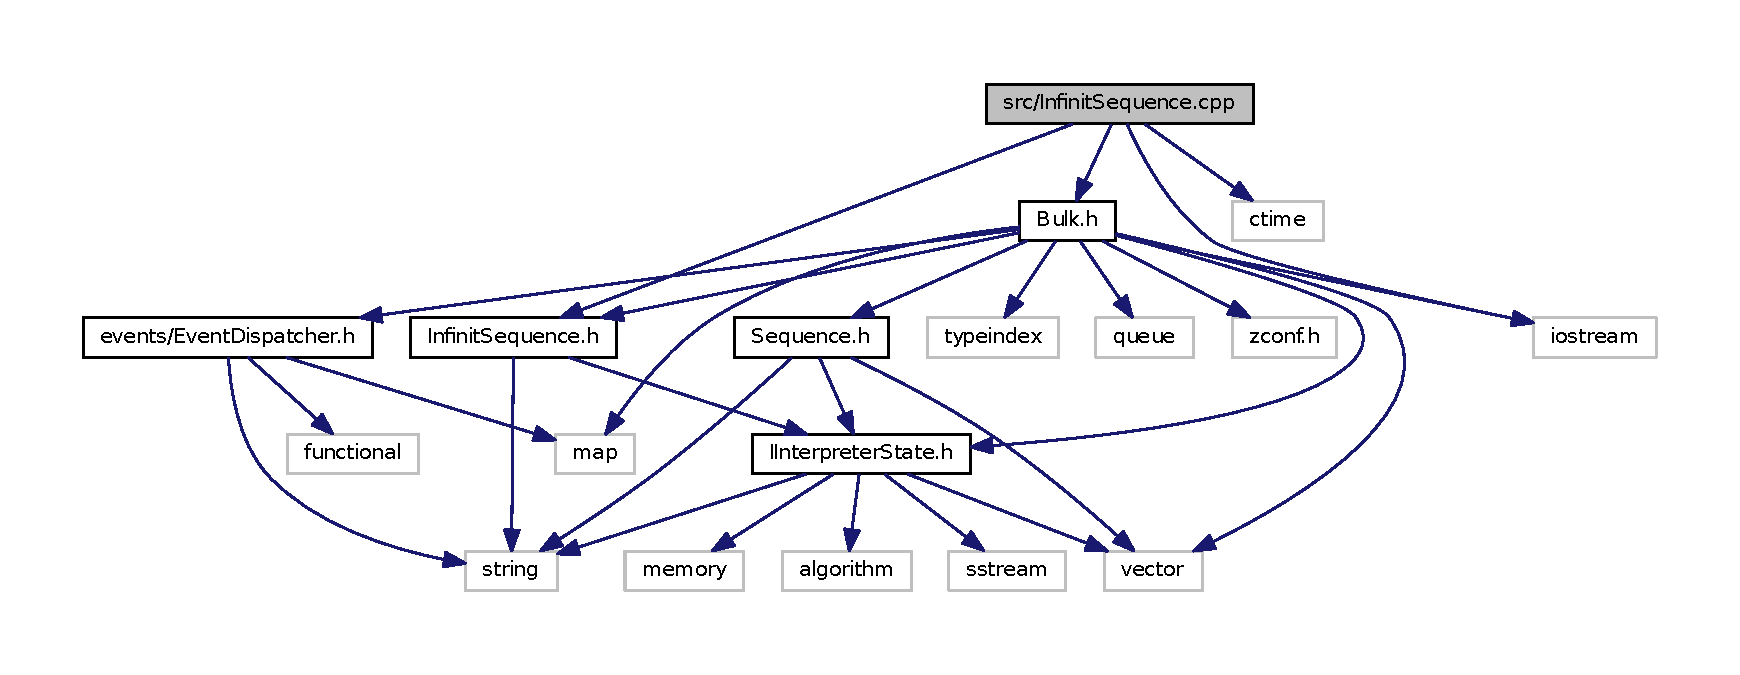
\includegraphics[width=350pt]{_infinit_sequence_8cpp__incl}
\end{center}
\end{figure}

\hypertarget{_infinit_sequence_8h}{}\section{src/\+Infinit\+Sequence.h File Reference}
\label{_infinit_sequence_8h}\index{src/\+Infinit\+Sequence.\+h@{src/\+Infinit\+Sequence.\+h}}
{\ttfamily \#include \char`\"{}I\+Interpreter\+State.\+h\char`\"{}}\\*
{\ttfamily \#include $<$string$>$}\\*
Include dependency graph for Infinit\+Sequence.\+h\+:
\nopagebreak
\begin{figure}[H]
\begin{center}
\leavevmode
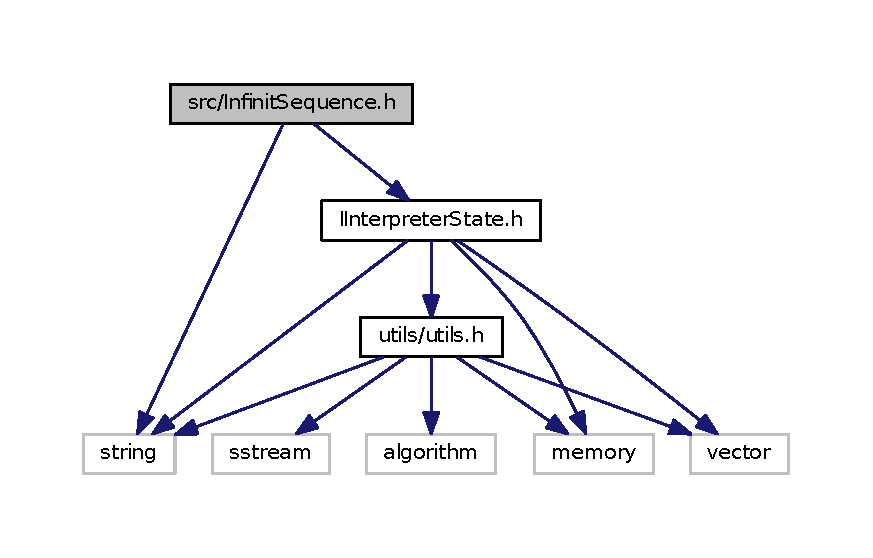
\includegraphics[width=350pt]{_infinit_sequence_8h__incl}
\end{center}
\end{figure}
This graph shows which files directly or indirectly include this file\+:
\nopagebreak
\begin{figure}[H]
\begin{center}
\leavevmode
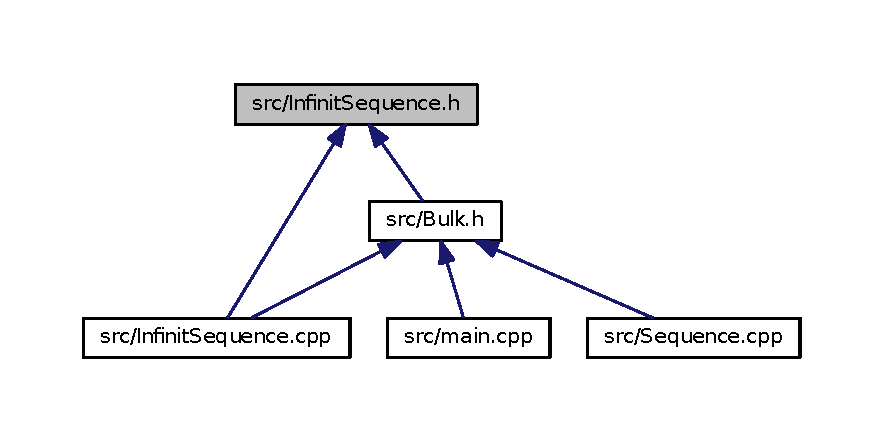
\includegraphics[width=350pt]{_infinit_sequence_8h__dep__incl}
\end{center}
\end{figure}
\subsection*{Classes}
\begin{DoxyCompactItemize}
\item 
class \hyperlink{class_infinit_sequence}{Infinit\+Sequence}
\end{DoxyCompactItemize}

\hypertarget{_console_logger_8h}{}\section{src/log/\+Console\+Logger.h File Reference}
\label{_console_logger_8h}\index{src/log/\+Console\+Logger.\+h@{src/log/\+Console\+Logger.\+h}}
{\ttfamily \#include $<$iostream$>$}\\*
{\ttfamily \#include $<$string$>$}\\*
Include dependency graph for Console\+Logger.\+h\+:
\nopagebreak
\begin{figure}[H]
\begin{center}
\leavevmode
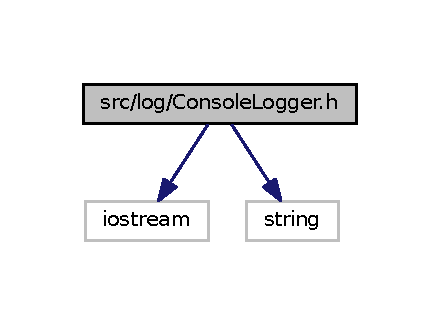
\includegraphics[width=211pt]{_console_logger_8h__incl}
\end{center}
\end{figure}
This graph shows which files directly or indirectly include this file\+:
\nopagebreak
\begin{figure}[H]
\begin{center}
\leavevmode
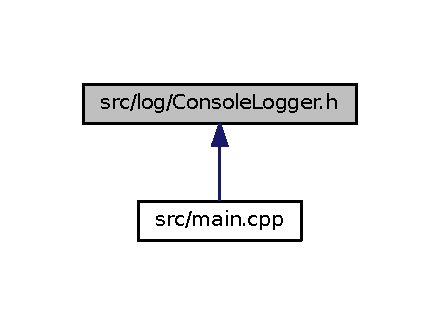
\includegraphics[width=211pt]{_console_logger_8h__dep__incl}
\end{center}
\end{figure}
\subsection*{Classes}
\begin{DoxyCompactItemize}
\item 
struct \hyperlink{struct_console_logger}{Console\+Logger}
\end{DoxyCompactItemize}

\hypertarget{_file_logger_8h}{}\section{src/log/\+File\+Logger.h File Reference}
\label{_file_logger_8h}\index{src/log/\+File\+Logger.\+h@{src/log/\+File\+Logger.\+h}}
{\ttfamily \#include $<$string$>$}\\*
{\ttfamily \#include $<$fstream$>$}\\*
Include dependency graph for File\+Logger.\+h\+:
\nopagebreak
\begin{figure}[H]
\begin{center}
\leavevmode
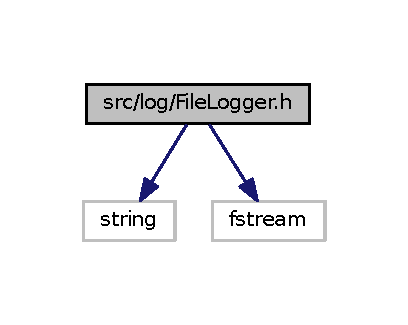
\includegraphics[width=196pt]{_file_logger_8h__incl}
\end{center}
\end{figure}
This graph shows which files directly or indirectly include this file\+:
\nopagebreak
\begin{figure}[H]
\begin{center}
\leavevmode
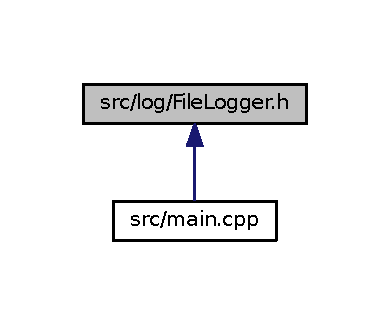
\includegraphics[width=187pt]{_file_logger_8h__dep__incl}
\end{center}
\end{figure}
\subsection*{Classes}
\begin{DoxyCompactItemize}
\item 
struct \hyperlink{struct_file_logger}{File\+Logger}
\end{DoxyCompactItemize}

\hypertarget{main_8cpp}{}\section{src/main.cpp File Reference}
\label{main_8cpp}\index{src/main.\+cpp@{src/main.\+cpp}}
{\ttfamily \#include $<$iostream$>$}\\*
{\ttfamily \#include $<$regex$>$}\\*
{\ttfamily \#include \char`\"{}Bulk.\+h\char`\"{}}\\*
{\ttfamily \#include \char`\"{}log/\+Console\+Logger.\+h\char`\"{}}\\*
{\ttfamily \#include \char`\"{}log/\+File\+Logger.\+h\char`\"{}}\\*
Include dependency graph for main.\+cpp\+:
\nopagebreak
\begin{figure}[H]
\begin{center}
\leavevmode
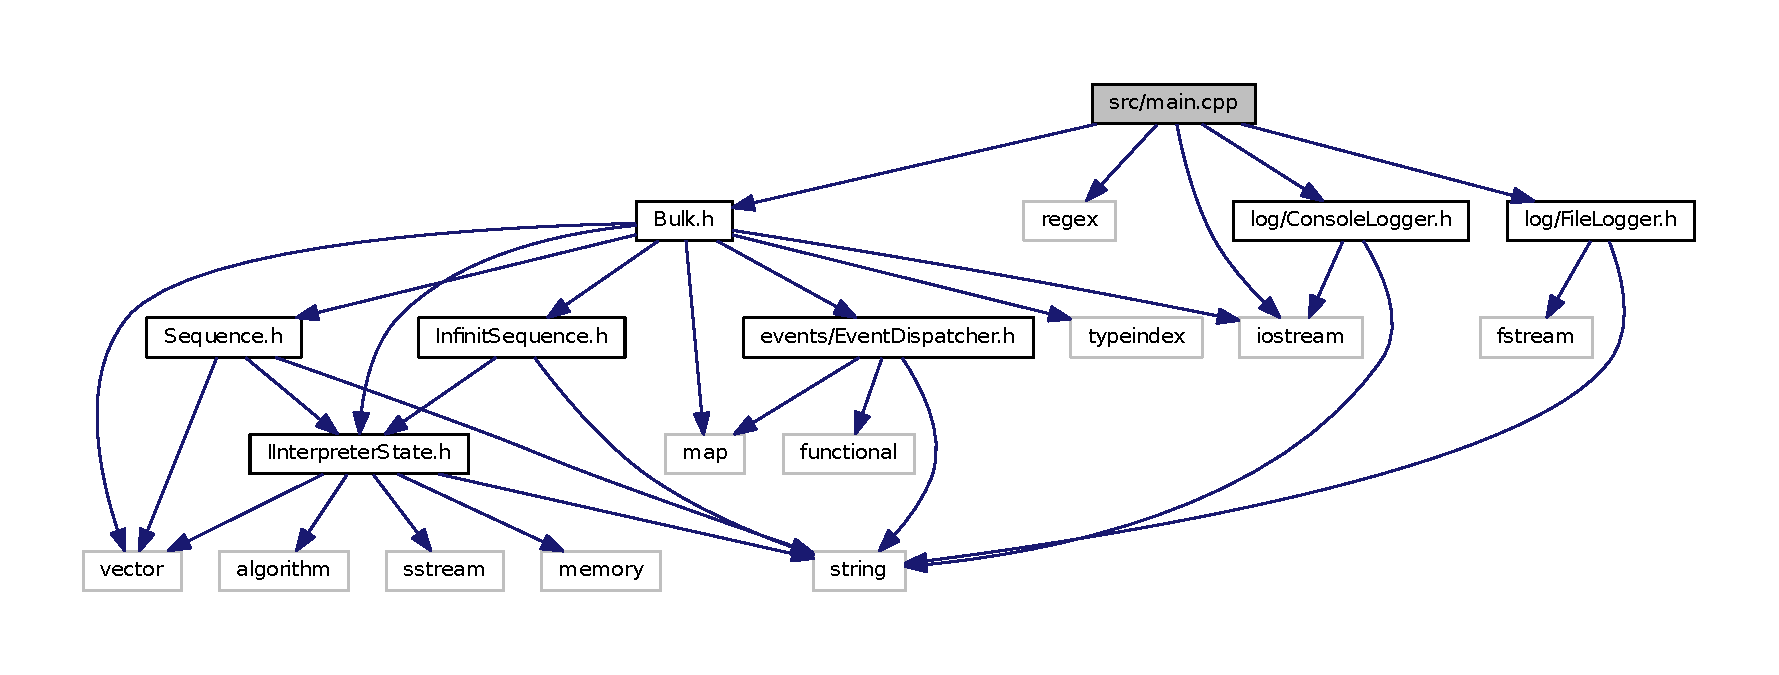
\includegraphics[width=350pt]{main_8cpp__incl}
\end{center}
\end{figure}
\subsection*{Functions}
\begin{DoxyCompactItemize}
\item 
int \hyperlink{main_8cpp_a44f39fa694ede1d31522a3d5bb38d6ba}{main} (int, char const $\ast$argv\mbox{[}$\,$\mbox{]})
\begin{DoxyCompactList}\small\item\em Main app function. \end{DoxyCompactList}\end{DoxyCompactItemize}


\subsection{Function Documentation}
\index{main.\+cpp@{main.\+cpp}!main@{main}}
\index{main@{main}!main.\+cpp@{main.\+cpp}}
\subsubsection[{\texorpdfstring{main(int, char const $\ast$argv[])}{main(int, char const *argv[])}}]{\setlength{\rightskip}{0pt plus 5cm}int main (
\begin{DoxyParamCaption}
\item[{int}]{, }
\item[{char const $\ast$}]{argv\mbox{[}$\,$\mbox{]}}
\end{DoxyParamCaption}
)}\hypertarget{main_8cpp_a44f39fa694ede1d31522a3d5bb38d6ba}{}\label{main_8cpp_a44f39fa694ede1d31522a3d5bb38d6ba}


Main app function. 


\hypertarget{_sequence_8cpp}{}\section{src/\+Sequence.cpp File Reference}
\label{_sequence_8cpp}\index{src/\+Sequence.\+cpp@{src/\+Sequence.\+cpp}}
{\ttfamily \#include \char`\"{}Sequence.\+h\char`\"{}}\\*
{\ttfamily \#include \char`\"{}Bulk.\+h\char`\"{}}\\*
{\ttfamily \#include $<$iostream$>$}\\*
{\ttfamily \#include $<$ctime$>$}\\*
Include dependency graph for Sequence.\+cpp\+:
\nopagebreak
\begin{figure}[H]
\begin{center}
\leavevmode
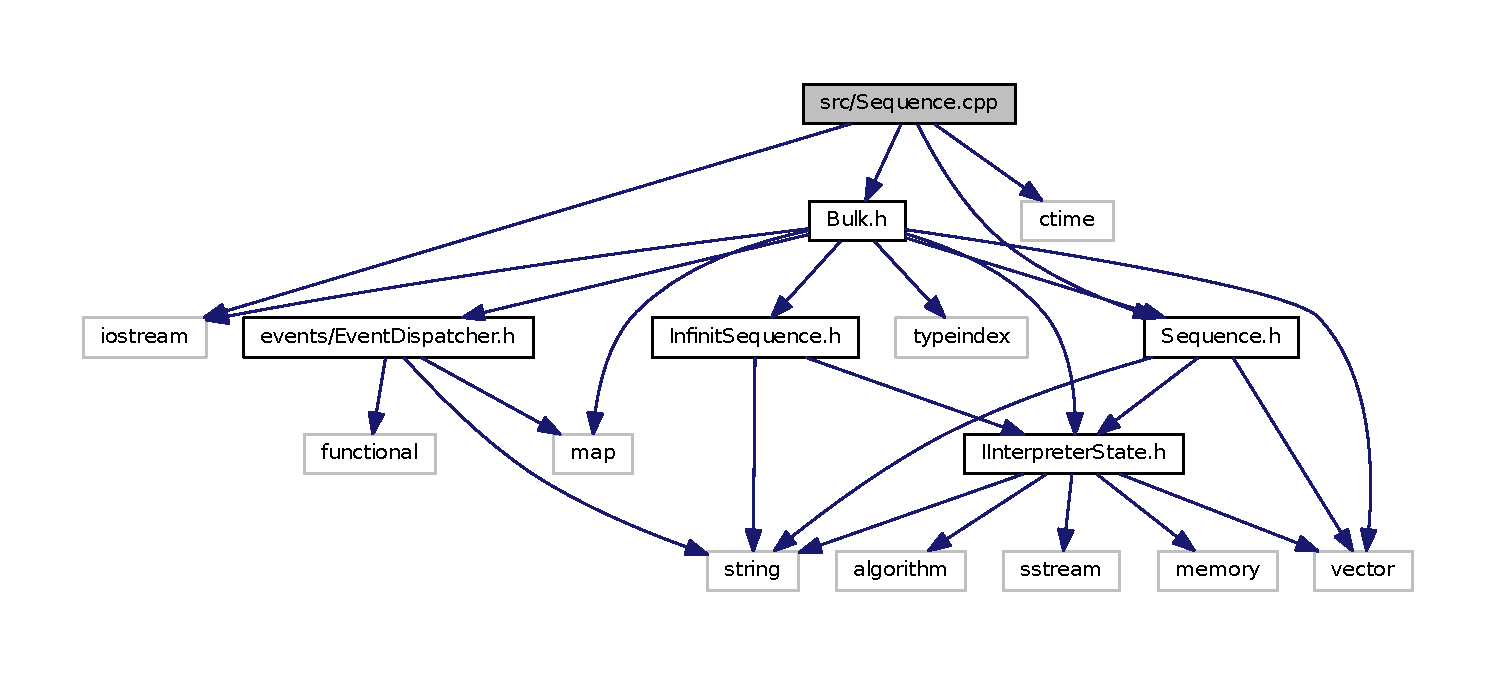
\includegraphics[width=350pt]{_sequence_8cpp__incl}
\end{center}
\end{figure}

\hypertarget{_sequence_8h}{}\section{src/\+Sequence.h File Reference}
\label{_sequence_8h}\index{src/\+Sequence.\+h@{src/\+Sequence.\+h}}
{\ttfamily \#include $<$string$>$}\\*
{\ttfamily \#include $<$vector$>$}\\*
{\ttfamily \#include \char`\"{}I\+Interpreter\+State.\+h\char`\"{}}\\*
Include dependency graph for Sequence.\+h\+:
\nopagebreak
\begin{figure}[H]
\begin{center}
\leavevmode
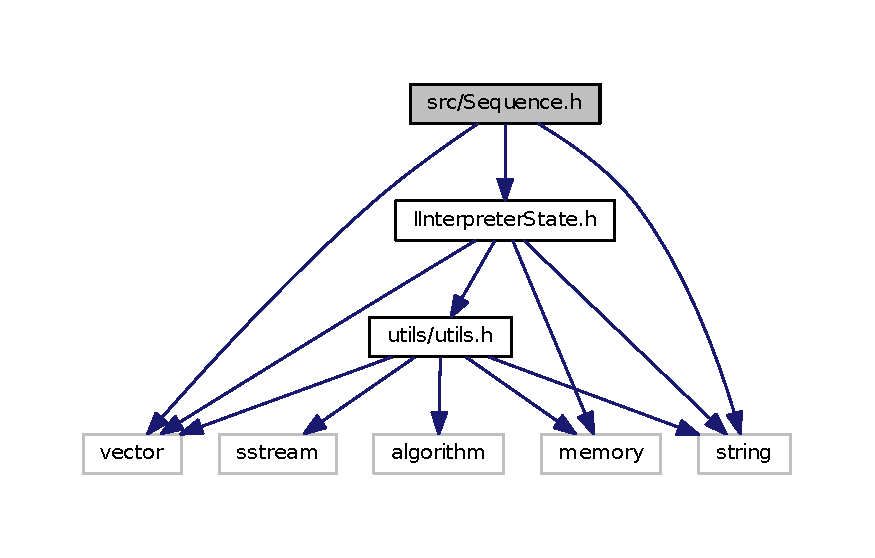
\includegraphics[width=350pt]{_sequence_8h__incl}
\end{center}
\end{figure}
This graph shows which files directly or indirectly include this file\+:
\nopagebreak
\begin{figure}[H]
\begin{center}
\leavevmode
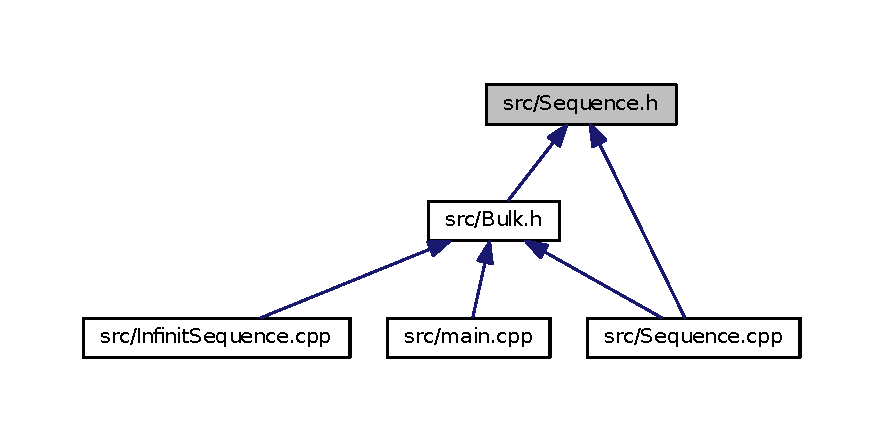
\includegraphics[width=350pt]{_sequence_8h__dep__incl}
\end{center}
\end{figure}
\subsection*{Classes}
\begin{DoxyCompactItemize}
\item 
class \hyperlink{class_sequence}{Sequence}
\end{DoxyCompactItemize}

\hypertarget{utils_8h}{}\section{src/utils/utils.h File Reference}
\label{utils_8h}\index{src/utils/utils.\+h@{src/utils/utils.\+h}}
{\ttfamily \#include $<$vector$>$}\\*
{\ttfamily \#include $<$string$>$}\\*
{\ttfamily \#include $<$sstream$>$}\\*
{\ttfamily \#include $<$memory$>$}\\*
{\ttfamily \#include $<$algorithm$>$}\\*
Include dependency graph for utils.\+h\+:
\nopagebreak
\begin{figure}[H]
\begin{center}
\leavevmode
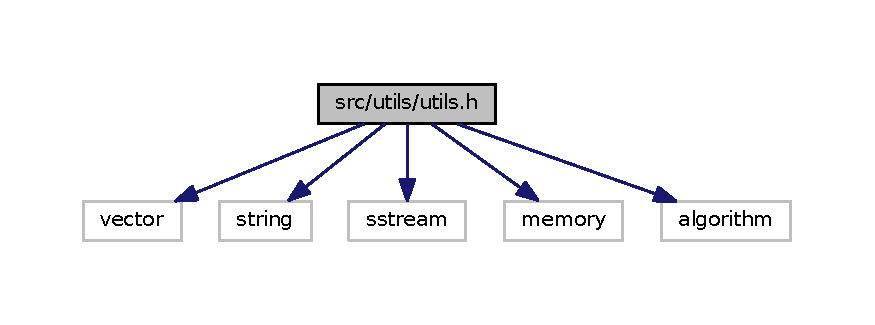
\includegraphics[width=350pt]{utils_8h__incl}
\end{center}
\end{figure}
This graph shows which files directly or indirectly include this file\+:
\nopagebreak
\begin{figure}[H]
\begin{center}
\leavevmode
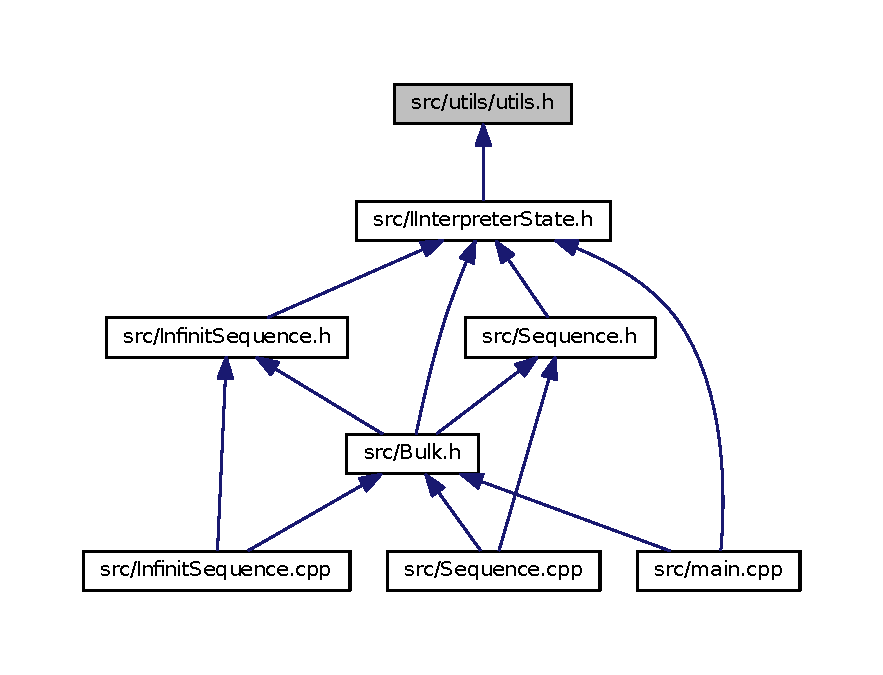
\includegraphics[width=350pt]{utils_8h__dep__incl}
\end{center}
\end{figure}
\subsection*{Namespaces}
\begin{DoxyCompactItemize}
\item 
 \hyperlink{namespace_utils}{Utils}
\end{DoxyCompactItemize}
\subsection*{Functions}
\begin{DoxyCompactItemize}
\item 
{\footnotesize template$<$typename T $>$ }\\std\+::string \hyperlink{namespace_utils_ac254de62ea3e311a2d9c6b9924cba1ee}{Utils\+::\+To\+String} (T value)
\item 
{\footnotesize template$<$typename T $>$ }\\std\+::string \hyperlink{namespace_utils_ae6413af43861acb7b4519bf17f777502}{Utils\+::\+To\+String} (std\+::shared\+\_\+ptr$<$ T $>$ value)
\item 
{\footnotesize template$<$class T $>$ }\\std\+::string \hyperlink{namespace_utils_a4b91cd26e4db77e0afb6fc34a0a5534e}{Utils\+::\+Join} (std\+::vector$<$ T $>$ container, std\+::string \&\&delimiter)
\end{DoxyCompactItemize}

%--- End generated contents ---

% Index
\backmatter
\newpage
\phantomsection
\clearemptydoublepage
\addcontentsline{toc}{chapter}{Index}
\printindex

\end{document}
